\documentclass[a4paper,12pt,dvipdfmx]{jsarticle_measlab}
\bibliographystyle{junsrt_KIT} 
\usepackage{layout}
\usepackage{amsmath}
\usepackage[dvipdfmx]{graphicx}
\usepackage{here} %画像位置
\usepackage{bm}
\usepackage{mathtools}
\usepackage{enumitem}
\setlist[description]{
  font={\normalfont}
}

\let\Re\relax
\DeclareMathOperator{\Re}{Re}
\let\Im\relax
\DeclareMathOperator{\Im}{Im}

% キャプションの設定を変更しないまま Subcaption を導入する.
\makeatletter
\let\MYcaption\@makecaption
\makeatother
\usepackage{subcaption}
\captionsetup{compatibility=false}      % 必要に応じて
\makeatletter
\let\@makecaption\MYcaption
\makeatother
\pagenumbering{roman}

\title{\LARGE Title 1}
\secondtitle{\LARGE Title 2}
\author{Your Name}
\date{5}
\studentid{Your Student Number}
\studentname{Your Name}
\teachername{田中 洋介 准 教 授}
\secondteachername{村田 滋 教 授}
% \studentid{\hspace{19pt}18123054\hspace{19pt}}
% \studentname{\hspace{19pt}中井 大 \hspace{19pt}}
% \teachername{\hspace{19pt}田中 洋介 准 教 授\hspace{19pt}}
% \secondteachername{\hspace{19pt}村田 滋 教 授\hspace{19pt}}

\pagenumbering{arabic} 

\begin{document}
% 卒業論文では英文アブストは必要ないので削除してください
\section*{Abstract}
This study proposes a method for detecting proximity droplet pairs by extracting local features in sparse droplet holograms instead of performing holographic reconstruction. First, the study formulates the local features on the spectral distribution of co-diameter proximity droplet holograms that have no depth direction distance. Then, the relationship between the geometric shape parameters of the local features and the distances between the droplets is illustrated. It is shown that proximity droplets can be detected by extracting local features on the spectral distribution. Second, a convolutional neural network-based image recognition model for detecting proximity droplet holograms is constructed using this property. Finally, the constructed model is used to perform inference on experimental data. Furthermore, the collision pair that led to coalescence is visualized using phase retrieval holography. It is shown that this method can be used to extract droplet collision and coalescence. If the method is further improved to achieve high-precision measurements, it will be possible to experimentally verify the collision efficiency in a turbulent field, thus contributing to the elucidation of cloud microphysical processes.
\newpage
\section*{概要}
本研究は,疎に分布する粒子ホログラムに対して像再生を行わず,局所特徴を抽出することで近接粒子組を検出する手法を提案する.はじめに,奥行方向距離を持たない同径近接粒子ホログラムのスペクトル分布上局所特徴を定式化し,局所特徴の幾何形状パラメータと粒子間距離の関係を示す.こうしてスペクトル分布上の局所特徴を抽出することで粒子近接を検出できることが示される.次に,この性質を用いて粒子ホログラムから近接検出を行う畳み込みニューラルネットワークベースの画像認識モデルを構築する.最後に,構築したモデルを用いて実験データに対する推論を行う.さらに,位相回復ホログラフィを用いて像再生し,併合に至った水滴組を可視化する.本手法によって水滴の衝突併合を抽出できることが示される.さらに手法の改善により高精度計測が可能になれば,乱流場における衝突効率を実験的に検証することで雲の微物理過程解明に寄与できる.

\newpage
\tableofcontents
\newpage
\pagenumbering{arabic} 
\section{緒言}
過去50年で気象災害の発生件数は5倍に増加し,気象災害による経済損失は世界全体で一日あたり3億8300万ドルに達する\cite{wmo2021}.損失や被害を最小化するためには国際的な減災対策が必要であり,その手段のひとつとして全球気候モデル\cite{climatemodel}や地球システムモデル\cite{earthsystem}による気候変動の将来予測が不可欠である.しかし,これらのモデルは一般に水平方向に\SI{100}{\km}ほどの格子解像度を有しており,雲内部の詳細な現象を計算し再現することは原理的に難しい\cite{grabowski2019}.雲粒の凝結や蒸発,衝突・併合による成長などといった,気候モデルの雲内部で再現できない微小スケールの物理現象を雲の微物理過程と呼ぶ.気候モデルにおいては雲の微物理過程の統計的な効果を経験的な近似手法であるバルク法で代替する\cite{kessler1969,lin1983,rutledge1984}.しかし,バルク法ではモデル全体の予測精度を向上させるために人為的なパラメータ調整が行われている\cite{hourdin2017}ため,線状降水帯などのメカニズムが未解明の降水現象や顕著気象に対する精度や信頼性の高い予測が困難である.したがって,気候モデルの精度・信頼性向上のために物理法則に基づく雲再現手法の開発が重要であり,そのために雲の微物理過程を解明することが課題である.

上記の課題解決のために,限定的な時空間領域における雲内部の現象を高い解像度で計算し再現する雲解像モデルを用いた研究が行われている\cite{khain2015,grabowski2019,morrison2020}.なかでも,確率的粒子法ベースの超水滴法\cite{shima2009,shima2020}は精度・性能ともに優れた雲解像モデルとして注目されている.超水滴法では,水滴・氷晶やエアロゾルなどの実粒子を,属性 $\bm{c}$ と多重度 $\xi$ を持つ仮想粒子である超水滴で代替する.属性 $\bm{c}$ は粒子の性質を,多重度 $\xi$ はその超水滴が表現する実粒子の個数を表す.超水滴同士の相互作用は確率モデルによって表現され,そのモンテカルロサンプリングによって時間発展を計算する.この手法は,雲の微物理過程を物理法則に基づいて解明するための有力な手段である.

超水滴法などの雲解像モデルで用いられる,水滴の併合による成長を記述する確率分布は,以下で与えられる\cite{gillespie1972,shima2020}.
\begin{equation}
    \label{intro:collisionprobability}
    P_{ij} = K(a_i, a_j) \frac{\mathrm{d}t}{\Delta V}
\end{equation}
$P_{ij}$は,領域$\Delta V$中にある半径 $a_i$ の水滴$i$と半径 $a_j$ の水滴$j$が,時間$\mathrm{d}t$の間に衝突・併合する確率を表す.$K(a_i,a_j)$は衝突併合カーネルと呼ばれ,系によっていくつかの表現があるものの,例えば無風状態で重力のみがはたらく理想的な状況では,以下のように与えられる\cite{pruppacher1996}.
\begin{equation}
    \label{intro:collisionkernel}
    % Pruppacker and Klett, Eq.(15-2)
    K(a_i, a_j) = E_{col}(a_i,a_j) \pi (a_i + a_j)^2 \left( U_{\infty,i} - U_{\infty,j} \right)
\end{equation}
ただし,$a_i>a_j$である.$U_{\infty}$は粒子の終端速度である.$E_{col}$は捕集効率(collection efficiency)と呼ばれ,水滴の水力学的相互作用を表す.半径が大きいコレクタ水滴の後流の影響で単純な剛体系として扱えないため重要である.捕集効率$E_{col}$は,さらに以下の衝突効率$E_{colli}$と併合効率$E_{coal}$に分解して表現できる.
\begin{equation}
    \label{intro:collectionefficiency}
    E_{col} = E_{colli} E_{coal}
\end{equation}
併合効率$E_{coal}$は,水滴組が衝突後併合へ至る割合で定義される.この系の衝突効率$E_{colli}$は,水滴$j$がコレクタ水滴$i$をかすめる水平オフセット$y_c$を用いて以下で定義される\cite{pruppacher1996}.
\begin{equation}
    \label{intro:collisionefficiency}
    E_{colli} = \frac{y_c}{\left( a_i + a_j \right) ^ 2}
\end{equation}
2つの水滴と$y_c$の関係をFig. \ref{fig:horizontaloffset}に示す.2つの水滴が十分な鉛直方向距離を持つとき,$y_c$はある値に収束し,小さな水滴$j$が$y_c$で定義する軌跡よりも内側にあれば,衝突が発生する.実際の$y_c$の値は理論的な解析や実験によって決定される.
\begin{figure}[b]
    \centering
    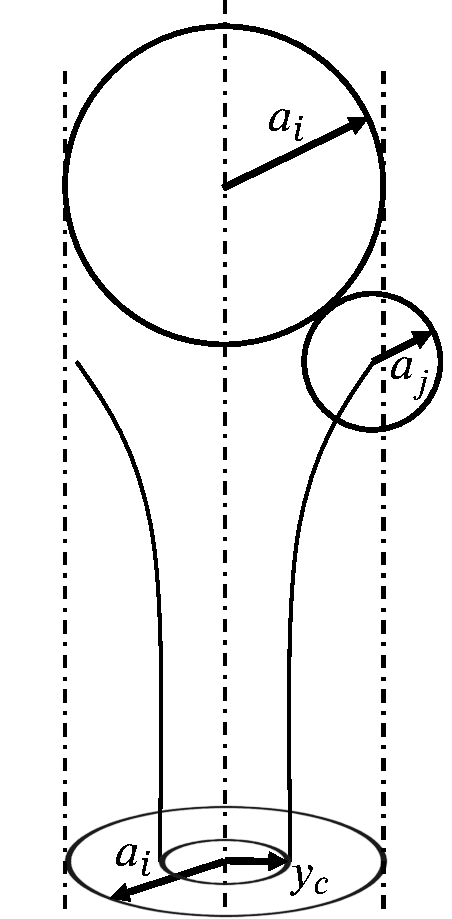
\includegraphics[width=0.4\linewidth]{./Figure/1_Introduction/yc.pdf}
    \caption{Schematic diagram of colliding droplet pair with horizontal offset for a grazing trajectory of the small droplet $y_c$; if the origin of the small droplet $j$ is inside the trajectory defined by $y_c$, the collision occurs.}
    \label{fig:horizontaloffset}
\end{figure}
無風状態や層流条件における衝突効率$E_{colli}$および併合効率$E_{coal}$の研究は2000年までにおおよそ完了しており,Pruppacher and Klett (1996)\cite{pruppacher1996}はその代表的な総説である.雲解像モデルにおける衝突併合モデルではDavis (1972)\cite{davis1972},Jonas (1972)\cite{jonas1972},Hall (1980)\cite{hall1980},Lin and Liu (1975)\cite{linliu1975}などの理論的な値を用いるか,Pinsky (2001)\cite{pinsky2001}の数値計算による導出が一般的である.超水滴法では前者の理論による値が用いられている.導出された分布は,風洞実験による結果との整合性が確認されている\cite{abbott1974, telford1955, woods1964}.

2000年頃から現在にかけては,実際の大気乱流条件におけるこれらの分布やその原理の解明が注目されている.乱流場における衝突・併合効率の研究は,主に層流条件における分布からの増加成分 $\Delta E$ について行われている.数値シミュレーションによる乱流場衝突効率の計算\cite{pinsky2008Part5},衝突効率の強化原理の説明\cite{pinsky2007Part4}などが行われ,実験では,風洞で生成した乱流場における衝突効率の測定値とその平均層流場との差が,乱流場における衝突効率の増加成分 $\Delta E_{colli}$ として報告されている\cite{vohl1999}.今後の乱流場における衝突・併合効率の研究で特に重要とされているのは,\SI{100}{\um}以上の水滴に対する衝突効率の評価と,水滴の分裂確率カーネルの導出である\cite{khain2018}.

以上より,筆者らの研究の最終的な目標は,乱流場における衝突・併合効率の実験的な検証および導出である.インラインホログラフィ\cite{gabor}を用いた3次元微粒子計測\cite{tanaka2016,kubonishi2018,nakatani2019}は,水滴の衝突・併合現象の直接的な観測に適している.また,GPUを用いた3次元像再生の高速化\cite{shimobaba2008, tanaka2019, nakai2022, tanaka2024}によって現実的な処理時間での計測が可能となった.これまで行われてきたホログラフィを用いた雲粒観測\cite{thompson1974,brown1989,fugal2009}では,雲粒の粒径分布や数密度などの統計量が得られているが,高速度撮影による衝突・併合現象の直接観測は行われていない.雲粒の高速度ホログラフィックイメージングは,雲粒の衝突・併合現象の直接観測とそれによる衝突・併合効率の評価を可能にする手法として期待される.

本研究では,高速度ホログラフィックイメージングによって水滴の衝突・併合効率の評価を行うために,ホログラフィを用いて水滴の衝突・併合現象を3次元観測するための手法の確立を目的とする.ホログラフィ計測でよく用いられる光波の逆伝搬による像再生は,GPUによって高速化されたもののその処理速度一枚あたり\SI{1.7}{s}ほどを要する\cite{nakai2022}.水滴の高速度撮影では\SI{4000}{fps}で撮影するため,衝突水滴を記録していないホログラムも含めてすべてのホログラムを像再生することは効率的ではない.したがって,はじめに本論文では,記録された粒子ホログラム画像から,ホログラム再生を行わず画像の局所特徴を直接抽出することで近接した粒子組を検出する手法を提案し,その原理を実験によって検証する\cite{nakai2023}.さらに,提案した原理を用いて設計した深層学習モデルによる画像認識を行い,実際に撮影した時系列水滴ホログラムから衝突水滴組を検出する.


本論文において,以降の各章で述べる内容を示す.第2章では,インラインホログラフィの原理,近接粒子ホログラムの理論,近接水滴抽出のための深層学習モデルの概要と,抽出したホログラムを像再生するために用いる位相回復ホログラフィの原理について説明する.第3章では,近接粒子ホログラムの局所特徴抽出のための検証実験,モデルの定義と学習方法,時系列水滴ホログラムの記録について述べる.第4章では,検証実験,モデルの学習,抽出結果の像再生それぞれについて結果を示し,考察を行う.第5章では,本論文の総括と結論を述べる.
\newpage
\section{理論}
\subsection{インラインホログラフィによる粒子の記録と3次元再生}\label{sec:in-lineHolography}
微小物体が存在する3次元空間を通過したコヒーレントな単一波長平行光波は,弱位相物体(weak phase object)による光路長の変化・屈折・反射や,あるいは不透明物体(opaque object)による部分的な遮光・周囲の回折などの作用によって変化する.この光波がさらに光軸方向に伝搬し,ある地点でイメージセンサなどによって光強度として記録されたとき,そのうち特に物体の存在によって生じる干渉・回折パターンをホログラムと呼ぶ.また,記録したホログラムから3次元物体像を復元する技術はホログラフィ\cite{gabor}を呼ばれる.光源・物体・記録媒体がすべて同一軸上にある光学系によるホログラフィは,Gaborによって発明されたことからGaborホログラフィ(Gabor's holography),あるいはインラインホログラフィ(in-line holography)と呼ばれる.

平面波の光伝搬はコンピュータで計算可能である\cite{kreis}ため,物体が存在する空間を通過して伝搬した光複素振幅を観測できれば,その光を物体が存在していた位置まで逆伝搬することで物体がある位置の複素振幅から物体の分布や形状を測定できる.ホログラムの干渉・回折パターンには,それを記録した地点の複素振幅が含まれる.以下では,コンピュータによる光複素振幅の伝搬計算,インラインホログラフィにおける物体の記録・再生方法について順に示す.

\subsubsection{単一波長平行光の伝搬計算}\label{sec:lightwaveProp}
この節では,ホログラムの記録とコンピュータによるホログラム再生の原理である光伝搬式とその計算について示す.光伝搬計算には,角スペクトル法\cite{goodman}を用いる.角スペクトル法は,光伝搬をフーリエ変換によって畳み込み積分として表現することで,光伝搬計算を高速化する手法である.また,記録される微粒子像のホログラムを理論的に扱うために,後にKirchhoff-Fresnel回折式の近似表現として導かれるFresnel回折積分\cite{kreis}についても示す.まずは,コンピュータでホログラム再生計算を行う際に用いる角スペクトル法について示す.角スペクトル法では,近軸近似が必要ないため非常に高精度かつ高速な計算が可能である.

% Goodman,早崎本による角スペクトル法の説明
波長$\lambda$の単色平行波$\psi(x,y;z)$は,以下のヘルムホルツ方程式に従う.
\begin{equation}
    \label{th:helmholtz}
    \nabla^2 \psi(x,y;z) + \left(\frac{2\pi}{\lambda} \right)^2 \psi(x,y;z) = 0
\end{equation}
$\psi(x,y;z)$の$x,y$に関する二次元フーリエ変換を$U(\alpha,\beta;z)$とすると,これらは以下の関係に従う.
\begin{align}
    \label{th:lightwaveFourier}
    U(\alpha,\beta;z) &= \mathcal{F}\{\psi(x,y;z)\} = \iint_{-\infty}^{\infty} \psi(x,y;z) \exp{\left(-2\pi \mathrm{j} (x\alpha + y\beta)\right)} \mathrm{d}x\mathrm{d}y \\
    \label{th:lightwaveInverseFourier}
    \psi(x,y;z) &= \mathcal{F}^{-1}\{U(\alpha,\beta;z)\} = \iint_{-\infty}^{\infty} U(\alpha,\beta;z) \exp{\left(2\pi \mathrm{j} (x\alpha + y\beta)\right)} \mathrm{d}\alpha\mathrm{d}\beta
\end{align}
ただし,$\alpha,\beta$はそれぞれ$x,y$のフーリエ変換空間の座標であり,$\mathrm{j}$は虚数単位である.式(\ref{th:lightwaveInverseFourier})を式(\ref{th:helmholtz})に代入すると,以下の式が得られる.

\begin{equation}
    \label{th:angularSpectrumequation}
    \frac{\partial^2 U(\alpha,\beta;z)}{\partial z^2} + \left( \frac{2 \pi}{\lambda} \right)^2 \left[ 1 - \left( \lambda \alpha \right)^2 - \left( \lambda \beta \right)^2 \right]U(\alpha,\beta;z) = 0
\end{equation}
式(\ref{th:angularSpectrumequation})の一般解として,以下の式が得られる.
\begin{equation}
    \label{th:angularSpectrumSolution}
    U(\alpha,\beta;z) = U(\alpha,\beta;0) \exp{\left( \frac{\mathrm{j}2\pi z}{\lambda} \sqrt{1-\left( \lambda \alpha \right)^2 - \left( \lambda \beta \right)^2} \right)}
\end{equation}
ここで,以下に定める関数 $G_z(\alpha,\beta)$ を角スペクトル法の伝達関数と呼ぶ.
\begin{equation}
    \label{th:angularSpectrumTransferFunction}
    G_z(\alpha,\beta) = \exp{\left( \frac{\mathrm{j}2\pi z}{\lambda} \sqrt{1-\left( \lambda \alpha \right)^2 - \left( \lambda \beta \right)^2} \right)}
\end{equation}
以上から,例えば$z=0$面から$z=z_0$面までの平行波の光伝搬は,以下のように計算できる.
\begin{equation}
    \label{th:lightProp_angularSpectrum}
    \psi(x,y,z_0) = \mathcal{F}^{-1}\left\{ \mathcal{F}\{\psi(x,y;0)\} \cdot \exp{\left( \frac{\mathrm{j}2\pi z_0}{\lambda} \sqrt{1-\left( \lambda \alpha \right)^2 - \left( \lambda \beta \right)^2} \right)} \right\}
\end{equation}
コンピュータで有限領域に対して離散的な平行波配列に対して上記の光伝搬計算を行う場合,以下の対応を用いる.
\begin{align}
    (x_i,y_j) &=  \left( i \Delta x , j\Delta y \right)\\
    (\alpha_i,\beta_j) &= \left( \frac{i}{L\Delta x} , \frac{j}{L\Delta y} \right)
\end{align}
ただし,$L$は離散フーリエ変換を行う配列の一辺の要素数である.また,$\Delta x$,$\Delta y$はそれぞれ$x$,$y$の離散化幅である.本研究でコンピュータを用いて行うホログラムの記録・再生に係る光伝搬計算は,すべて上記の角スペクトル法を用いる.

次に,Fresnel-Kirchhoff回折式から従うFresnel回折積分による光伝搬計算について示す.これは,後に理論的な粒子のホログラムを取り扱う際に必要となる.$z=0$面の単色平行光$\psi(x,y;0)$と,これが$z = z_0$面まで伝搬した複素振幅$\psi(x,y;z_0)$は,Fresnel-Kirchhoff回折式により以下の関係を満たす\cite{kreis}.
\begin{equation}
    \label{th:fresnel-kirchhoff}
    \psi(x,y;z_0) = \iint_{-\infty}^{\infty} \psi(x',y';0)\frac{z_0\exp{(\mathrm{j}2\pi r' /\lambda})}{\mathrm{j}\lambda r'^2} \mathrm{d}x'\mathrm{d}y'
\end{equation}
ただし,$r'=\sqrt{(x-x')^2+(y-y')^2+z_0^2}$である.ここで,系が以下の条件を満たすと仮定する.
\begin{equation}
    \label{th:fraunhoferCondition}
    \frac{\pi }{\lambda z_0} \left( {x'}_{\mathrm{max}}^2 + {y'}_{\mathrm{max}}^2 \right) \ll 1
\end{equation}
ただし,${x'}_{\mathrm{max}}$,${y'}_{\mathrm{max}}$は,$(x',y')$面の開口部,あるいは物体像座標の最大値である.この仮定のもと,$r'$を以下のように近似する.
\begin{align}
    r' &= \sqrt{(x-x')^2+(y-y')^2+z_0^2} \\
    &= z_0 \sqrt{1 + \frac{(x-x')^2+(y-y')^2}{z_0^2}} \\
    \label{th:approxOfR}
    &\approx z_0 \left( 1 + \frac{(x-x')^2+(y-y')^2}{2z_0^2} \right)
\end{align}
式(\ref{th:approxOfR})を式(\ref{th:fresnel-kirchhoff})に代入すると,以下のようになる\cite{tyler1976}.
\begin{equation}
    \label{th:fresneldiffraction}
    \psi(x,y;z_0) = \frac{\exp{ \left\{\mathrm{j}2\pi z_0 /\lambda \right\}}}{\mathrm{j}\lambda z_0} \iint_{-\infty}^{\infty} \psi(x',y';0)\exp{\left\{ \mathrm{j}\pi \frac{(x-x')^2+(y-y')^2}{z_0\lambda} \right\}} \mathrm{d}x'\mathrm{d}y'
\end{equation}
式(\ref{th:fresneldiffraction})を,Fresnel回折積分と呼ぶ.

\subsubsection{粒子ホログラムの記録}
\ref{sec:lightwaveProp}節で示した光伝搬計算を用いて,インラインホログラフィによる粒子像の記録を行う.インラインホログラフィにおける物体面,記録面の関係を図\ref{fig:in-lineHolography}に示す.ただし,物体面を表現する$(x',y')$座標は,式(\ref{th:fresnel-kirchhoff})のように回折積分の積分変数として記録面の$(x,y)$座標と区別する必要があるときだけ用いることとする.物体面および記録面で座標の単位長さは等しく,デカルト座標系を用いるため,これらを上に述べた理由以外で区別する必要はない.

\begin{figure}[htbp]
    \centering
    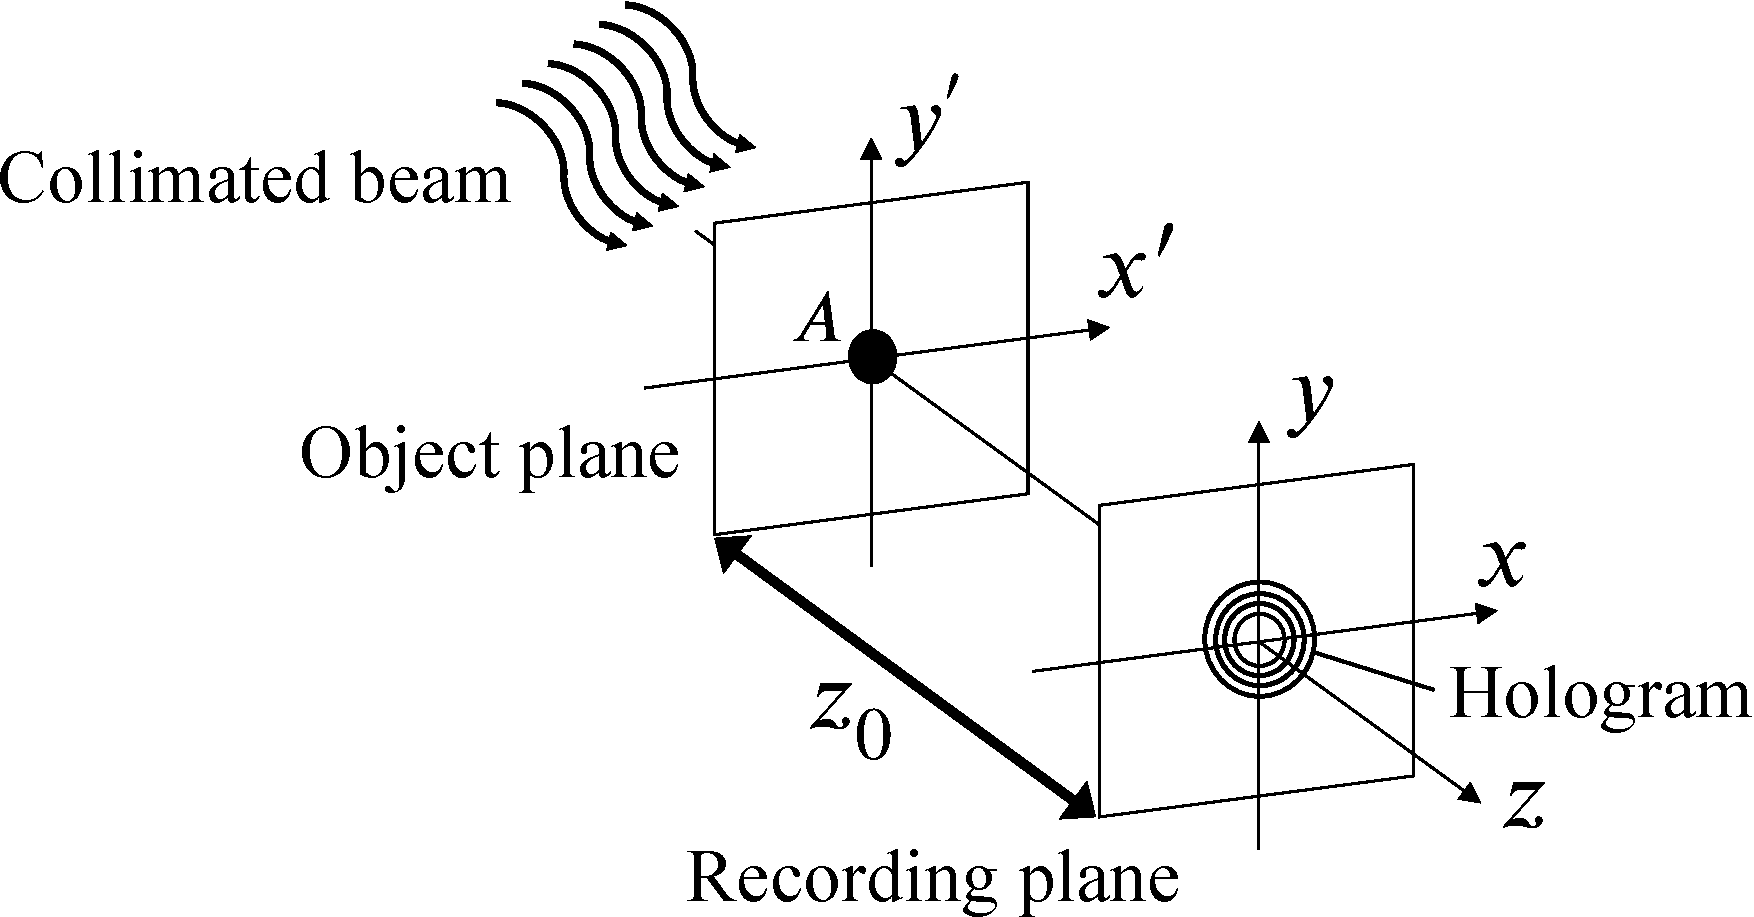
\includegraphics[width=0.8\linewidth]{./Figure/2_Theory/inline_holography.pdf}
    \caption{Schematic of in-line holography: collimated light illuminates a particle on the object plane, and appears as a diffraction pattern  on the recording plane. The irradiance of the complex amplitude on the recording plane is recorded as a hologram.}
    \label{fig:in-lineHolography}
\end{figure}

球形の3次元粒子は,ホログラムの記録時は3次元粒子中心に存在する物体面内の2次元円形として扱う.すなわち,$(x_p,y_p,z_p)$中心の半径 $a$の円は,以下の $z=z_p$上の形状関数$A(x,y;z_p)$として表現する.
\begin{equation}
    \label{th:particleShapeFunction}
    A(x,y;z_p) = \left\{
    \begin{aligned}
        &1 \quad \text{for } r_p \leq a \\
        &0 \quad \text{for } r_p > a
    \end{aligned}
    \right.
\end{equation}
ただし, $r_p=\sqrt{(x-x_p)^2+(y-y_p)^2}$である.今後この節では,便利のために$(x_p,y_p) = (0,0)$,$z_p = 0$とする.物体面$z=0$におけるコヒーレントな平行光の振幅を1,位相を0とすると,物体面における光複素振幅$\psi(x,y;0)$は,以下のようになる.
\begin{align}
    \psi(x,y;0) &= T(x,y)\cdot e^{\frac{2\pi \mathrm{j}}{\lambda}\cdot 0} \\
    &= 1 - A(x,y;0)
\end{align}
ここで,$T(x,y) = 1 - A(x,y;0)$は,物体面における透過関数と呼ばれる.これを$z_0$だけ伝搬して記録面の複素振幅$\psi(x,y;z_0)$を計算すると,式(\ref{th:fresneldiffraction}) に示すFresnel回折積分を用いて以下のようになる\cite{vikram}.
\begin{align}
    \label{th:particleComplexAmplitude}
    \psi(x,y;z_0) &= -\exp{\left( \frac{2\pi \mathrm{j}}{\lambda |z_0|} \right)} \left\{  
        1 + \frac{\mathrm{j}}{\lambda |z_0|} \exp{\left[ \frac{\pi \mathrm{j} \left( x^2+y^2 \right)}{\lambda |z_0|}\right] \tilde{A}\left( \frac{x}{\lambda |z_0|}, \frac{y}{\lambda |z_0|} \right) }
     \right\}
\end{align}
ただし, $\tilde{A}$は形状関数のフーリエ変換であり,以下の実数値関数で与えられる.
\begin{equation}
    \label{th:fourierOfA}
    \tilde{A}(\alpha,\beta) = \mathcal{F}\left\{ A \right\} = \pi a^2 \frac{2J_1(2\pi a \gamma)}{2\pi a \gamma}
\end{equation}
ここで, $\gamma = \sqrt{\alpha^2+\beta^2}$である.式(\ref{th:particleComplexAmplitude})では,以下の形式で用いられる.
\begin{equation}
    \label{th:fourierOfA2}
    \tilde{A}\left( \frac{x}{\lambda |z_0|}, \frac{y}{\lambda |z_0|} \right)  =  \pi a^2 \frac{2J_1(2\pi a r/ \lambda |z_0|)}{2\pi a r/ \lambda |z_0|}
\end{equation}
ただし, $r=\sqrt{x^2+y^2}$である.結局,式(\ref{th:particleComplexAmplitude})は以下のようになる.
\begin{equation}
    \label{th:particleComplexAmplitude2}
    \psi(x,y;z_0) = -\exp{\left( \frac{2\pi \mathrm{j}}{\lambda |z_0|} \right)} \left\{  
        1 + \frac{\mathrm{j}}{\lambda |z_0|} \exp{\left[ \frac{\pi \mathrm{j} \left( x^2+y^2 \right)}{\lambda |z_0|}\right] \pi a^2 \frac{2J_1(2\pi a r/ \lambda |z_0|)}{2\pi a r/ \lambda |z_0|} }
     \right\}
\end{equation}

記録面のホログラム$I(x,y)$は,複素振幅の強度の2乗として以下のように計算できる.
\begin{equation}
    \label{th:irradiance}
    I(x,y) = |\psi(x,y;z_0)|^2 = \psi(x,y;z_0)\psi^*(x,y;z_0)
\end{equation}
これに式(\ref{th:particleComplexAmplitude})を代入して,以下を得る\cite{tyler1976}.
\begin{equation}
    \label{th:particleIrradiance}
    I(x,y) = 1 - \frac{2\pi a^2}{\lambda |z_0|} \sin{\left( \frac{\pi r^2}{\lambda |z_0|} \right)} \frac{2J_1(2\pi ar/\lambda |z_0|)}{2\pi ar / \lambda |z_0|} + \left( \frac{\pi a^2}{\lambda |z_0|} \right)^2 \left[ \frac{2J_1(2\pi ar/\lambda |z_0|)}{2\pi ar / \lambda |z_0|} \right]
\end{equation}

\subsubsection{粒子ホログラムの再生}\label{sec:holographicReconstruction}
\ref{sec:lightwaveProp}節で示した光伝搬計算を用いて,インラインホログラフィによる粒子像の再生を行う.ここで,ある平面波 $u(x,y;z)$ の光伝搬を $u*h_z$ のように表現する.光伝搬の演算 $*h_z$ は,その物理的性質から以下を満たす.
\begin{align}
    \label{th:lightPropOperation}
    \left( u * h_{z_1} \right) * h_{z_2} = u * h_{z_1 + z_2}
\end{align}
また,式(\ref{th:angularSpectrumTransferFunction}),式(\ref{th:fresnel-kirchhoff})より,以下を満たす.
\begin{equation}
    \label{th:lightPropOperation2}
    \overline{h_z} = h_{-z}
\end{equation}
形状関数 $A$ を持つ物体のホログラムは以下で表現される\cite{scott1987}.
\begin{align}
    \label{th:abstructParticleHologram}
    I(x,y) &= \left| \left( 1 - A(x,y) \right) * h_{z_0} \right|^2 \\
    &= \left|  1 - A(x,y)  * h_{z_0} \right|^2 \\
    \label{th:abstructParticleHologram2}
    &= 1 - \overline{A(x,y)}*\overline{h_{z_0}} - A(x,y)*h_{z_0} + \left| A(x,y) * h_{z_0} \right|^2
\end{align}
ここで,$1*h_{z_0}=1$ を用いたが,これは物体面における平行光の位相を $-2\pi z_0 /\lambda$ とすることで成立する.これはのちの計算を簡単にするための操作であり,このような位相のずれを導入してもホログラムおよびその再生像には影響しない.また,式(\ref{th:abstructParticleHologram2})の右辺第3項は十分小さいため省略する.ホログラムを $-z_0$ だけ逆伝搬して物体面の複素振幅を計算することで,物体の再生像を得る.
\begin{align}
    \label{th:particleReconstruction}
    \psi_{rec}(x,y;0) &= I(x,y) * h_{-z_0} \\
    &= 1 - \overline{A(x,y)}*\overline{h_{z_0}}*h_{z_0} - A(x,y)*h_{z_0}*h_{z_0} \\
    &= 1 - \overline{A(x,y)} - A(x,y)*h_{2z_0} \\
    \label{th:particleReconstruction2}
    &= \left( 1 - A(x,y) \right) + (1 - A(x,y))*h_{2z_0} - e^{\frac{2\pi \mathrm{j}z_0}{\lambda}}
\end{align}
ただし,$A(x,y)$が実数値関数であることを用いた.式(\ref{th:particleReconstruction2})の第1項は物体光を,第2項は双画像を,第3項は背景光を表す.双画像はホログラム記録時に位相分布が失われることで生じる.双画像はインラインホログラフィでは原理的に除去できず,ノイズとして扱われる.

\subsubsection{ホログラフィによる計測精度のボトルネック}\label{sec:holographyBottleNeck}
前節の最後では,インラインホログラフィにおける像再生において,ホログラム記録時に位相分布が失われることで双画像が生じることを述べた.この節では,ホログラム計測においてその精度や像品質を低下させる典型的な問題である,双画像問題\cite{kats2010}と奥行方向への像伸び問題\cite{meng1995}について述べる.

本研究のように不透明物体を物体面上の形状関数で表現する場合,双画像による影響は再生時の物体輝度値変化として現れる.記録したホログラムを物体面まで逆伝搬して得た再生像スライスをFig. \ref{fig:twinImage:holo}に,その輝度分布を Fig. \ref{fig:twinImage:profile}に示す.Fig. \ref{fig:twinImage:profile}にはさらに,物体面の透過関数プロファイルも併せて示す.透過関数分布では,定義により粒子像の輝度値は0である.しかし,位相情報が失われたGaborホログラムの再生像では,双画像の影響により粒子輝度値が0でなくなる.さらに,双画像のホログラムフリンジも重畳しノイズとして再生像品質を低下させる.
\begin{figure}[htbp]
    \centering
    \begin{subfigure}[t]{0.48\linewidth}
        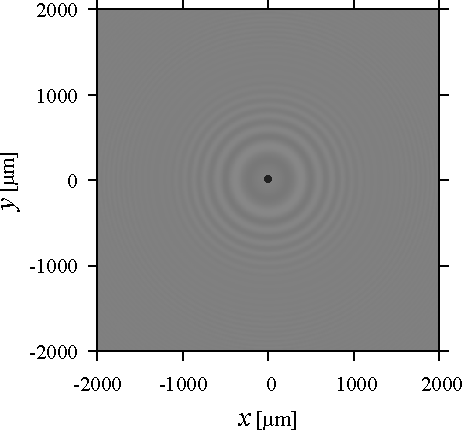
\includegraphics[width=\linewidth]{./Figure/2_Theory/twin_image/holo.pdf}
        \caption{Reconstructed image of Gabor hologram}
        \label{fig:twinImage:holo}
    \end{subfigure}
    \hfill
    \begin{subfigure}[t]{0.48\linewidth}
        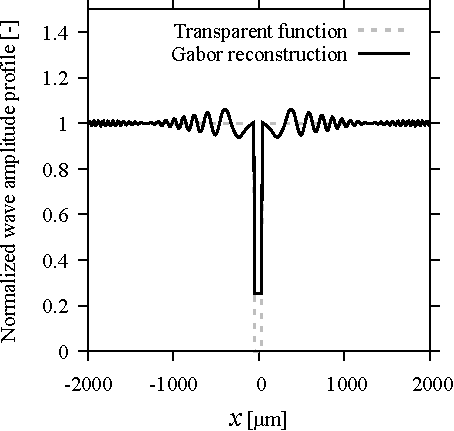
\includegraphics[width=\linewidth]{./Figure/2_Theory/twin_image/profile.pdf}
        \caption{Normalized wave amplitude profile of Gabor hologram and propagated wavefront along the line $y=\SI{0}{\um}$ }
        \label{fig:twinImage:profile}
    \end{subfigure}

    \caption{Example of a reconstructed image slice of Gabor hologram and its wavefront irradiance profile. The hologram is recorded at $z=\SI{80}{\mm}$, and the image slice is reconstructed at $z=\SI{0}{\mm}$. The particle radius is $a=\SI{50}{\um}$, and the recording wavelength is $\lambda = \SI{632.8}{\nm}$. The reconstructed particle image of the Gabor hologram does not have an amplitude of zero.}
    \label{fig:twinImage}
\end{figure}

次に,奥行方向への像伸び問題について述べる.記録ホログラムを再生して粒子座標を取得するとき,一般に粒子の奥行方向位置 $z_0$ は未知である.したがって,$x$-$y$ 投影像における粒子周辺の輝度分布の$z$ 軸プロファイルから $z_0$ を推定する必要がある.式(\ref{th:particleShapeFunction})に示す形状関数 $A$ で定義される粒子の $z$ 軸輝度プロファイルは,以下で与えられる\cite{born1970,tanaka2024}.
\begin{equation}
    \label{th:particleZprofile}
    I_z(z) := \left| \psi(0,0;z) \right|^2 \approx \left[ 1 + \cos{\left( \frac{\pi r_p^2}{\lambda z} \right)} \right]^2 + \sin^2{\left( \frac{\pi r_p^2}{\lambda z} \right)}
\end{equation}
Gaborホログラムの再生像のz軸輝度プロファイルと,式(\ref{th:particleZprofile})によるプロットをFig. \ref{fig:particleZprofile}に示す.
\begin{figure}[htbp]
    \centering
    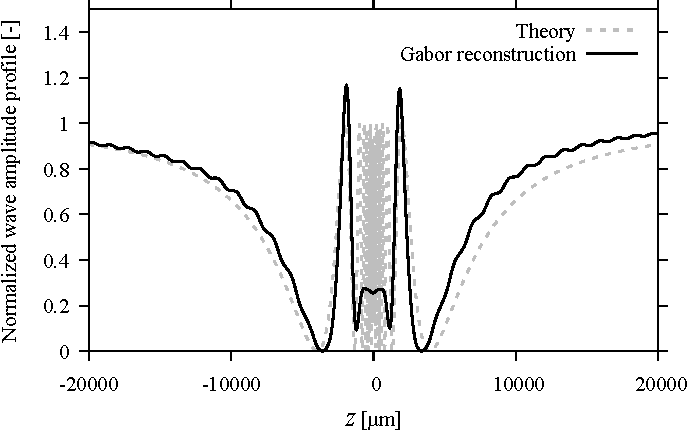
\includegraphics[width=0.8\linewidth]{./Figure/2_Theory/zprofile.pdf}
    \caption{Normalized $z$-axis irradiance profile of Gabor hologram and theoretical plot of Eq. (\ref{th:particleZprofile}). The hologram is recorded at $z = \SI{0}{\um}$, particle radius is $a=\SI{50}{\um}$, and the recording wavelength is $\lambda = \SI{632.8}{\nm}$. The same system used in Fig. \ref{fig:twinImage} is used for this calculation.}
    \label{fig:particleZprofile}
\end{figure}
式(\ref{th:particleZprofile})に示すプロファイルの,粒子$z$座標$z=0$に対して対象な零点間距離 $\Delta L$ は以下で与えられる\cite{nakatani2019}.
\begin{equation}
    \label{th:elongationLength}
    \Delta L = \frac{4r_p^2}{2(2n-1)\lambda}, \quad (n=1,2,3,\cdots)
\end{equation}
記録時に位相情報を失うインラインホログラフィによる再生では,$n=1$ は理論値を再現するもののそれより大きい $n$ では異なる.特に,$z=0$ における輝度値が双画像問題により0でなくなるため像抽出が困難になる.もし位相分布を復元してホログラムを再生できれば,後に示すように $n=0$ を中心として輝度値が 0 となる領域を抽出することができ,この領域に対する画像処理で粒子座標 $z$ を推定することができる.


双画像の影響は,再生波面から共役像項を除去したり,記録波面の位相分布を再生するなどして除去される.このために,Off-axis法\cite{offaxis}や位相シフト法\cite{phaseshift},Gerchberg-Saxtonアルゴリズムを用いた位相回復法\cite{phaseretrieval}などが用いられる.本研究では,後に示すように2台のカメラを用いた位相回復ホログラフィによってこれに対処する.


\subsection{2粒子ホログラムの局所特徴}\label{sec:twoParticleHologramFeature}
この節では,中心座標が $(x_{p1},y_{p1},z_{p1})$,半径 $a_1$ の粒子1と,中心座標が$(x_{p2},y_{p2},z_{p2})$,半径 $a_2$ の粒子2が近接したときに記録されるホログラフィックパターンの局所特徴について述べる.局所特徴とは画像上のある領域における幾何的な特徴を指す.すなわち,\ref{sec:holographicReconstruction}節で示したホログラムの3次元再生を行わず,ホログラムの画像としての特徴から直接粒子組の近接状態を識別することを目的とする.

\subsubsection{同径かつ奥行方向距離を持たない2粒子のホログラムとそのスペクトル分布}\label{sec:twoParticleHologram}
最も単純な場合として,2粒子が同じ半径 $a$ を持ち,かつ$z$軸方向距離を持たない場合を考える.すなわち,以下の条件を満たす.
\begin{align}
    \sqrt{(x_{p1}-x_{p2})^2+(y_{p1}-y_{p2})^2} > a_1+a_2  \quad &\text{条件1: 点間の距離が半径の和より大きい} \\
    a_1 = a_2 \quad &\text{条件2: 二つの半径が等しい} \\
    z_{p1} = z_{p2} \quad &\text{条件3: 同じz座標上にある}
\end{align}
粒子1の形状関数を $A_1$,粒子2の形状関数を $A_2$ とする.形状関数 $A_i$ は,式(\ref{th:particleShapeFunction})にならって以下のように定義する.
\begin{equation}
    \label{th:eachParticleShapeFunction}
    A_i(x,y;z_{pi}) = \left\{
    \begin{aligned}
        &1 \quad \text{for } \sqrt{(x-x_{p2})^2+(y-y_{p2})^2} \leq a \\
        &0 \quad \text{for } \sqrt{(x-x_{p2})^2+(y-y_{p2})^2} > a
    \end{aligned}
    \right.
\end{equation}
これらの光伝搬による記録ホログラムを計算する.
\begin{align}
    \psi_{z_0} &= \mathcal{F}^{-1}\left\{ \mathcal{F}\{(1-A_1)(1-A_2)\}G(\alpha,\beta;z_{p1}) \right\} \\
    &= \mathcal{F}^{-1}\left\{ \mathcal{F}\{(1-A_1)+(1-A_2)-1\}G(\alpha,\beta;z_{p1}) \right\} \\
    & \begin{multlined} = \mathcal{F}^{-1}\left\{ \mathcal{F}\{1-A_1\}G(\alpha,\beta;z_{p1}) \right\} + \mathcal{F}^{-1}\left\{ \mathcal{F}\{1-A_2\}G(\alpha,\beta;z_{p1}) \right\} \\ - \mathcal{F}^{-1}\left\{ \mathcal{F}\{1\}G(\alpha,\beta;z_{p1}) \right\} \end{multlined}
\end{align}
ここで, $\mathcal{F}^{-1}\left\{ \mathcal{F}\{1-A_i\}G(\alpha,\beta;z_{p1}) \right\}$ は形状関数 $A_i$ を持つそれぞれの粒子が単独で光伝搬した際の複素振幅と等しい.また  $\mathcal{F}^{-1}\left\{ \mathcal{F}\{1\}G(\alpha,\beta;z_{p1}) \right\}$ は背景光の光伝搬を示す.それぞれは式(\ref{th:particleComplexAmplitude})より以下のように計算できる.
\begin{equation}
    \label{th:vikramEq4.8}
    \psi_{pi}(x,y) = -\exp{\left(\mathrm{j}\frac{2\pi}{\lambda}|z_{pi}|\right)} \left\{ 1 + \frac{\mathrm{j}}{\lambda |z_{pi}|} \exp{ \left[ \frac{\mathrm{j} \pi \left( x'^2 + y'^2 \right)}{\lambda |z_{pi}|} \right]} \tilde{A_1} \left(\frac{x'}{\lambda |z_{pi}|},\frac{y'}{\lambda |z_{pi}|} \right)  \right\}
\end{equation}
% vikram 4.8 式
ただし, $x' = x- x_{pi}$, $y' = y-y_{pi}$ である.また,背景光の光伝搬 $\mathcal{F}^{-1}\left\{ \mathcal{F}\{1\}G(\alpha,\beta;z_{p1}) \right\}$ は以下のようになる.
\begin{equation}
    \psi_b(x,y) = \mathcal{F}^{-1}\left\{ \mathcal{F}\{1\}G(\alpha,\beta;z_{p1}) \right\} = \exp{\left(\frac{2\pi \mathrm{j}z_{p1}}{\lambda}\right)}
\end{equation}

さて,今の条件を満たす任意の系は,一方の粒子の中心が $(x,y)$ 平面上の原点に存在するよう座標変換可能である.原点に固定した粒子を粒子1と呼び,他方の粒子を粒子2と呼ぶ.また,粒子2の中心座標は $(\Delta \xi, \Delta \eta)$ とする.すなわち,以下を満たす.
\begin{align}
    \left( x_{p1}, y_{p1} \right) &= (0,0) \\
    \left( x_{p2}, y_{p2} \right) &= (\Delta \xi ,\Delta \eta)
\end{align}
このように定めた粒子1の複素振幅を $\psi_{A_1}$,粒子2の複素振幅を $\psi_{A_1}$ とする.系をFig. \ref{fig:twoParticleHolography}に示す.

\begin{figure}[htbp]
    \centering
    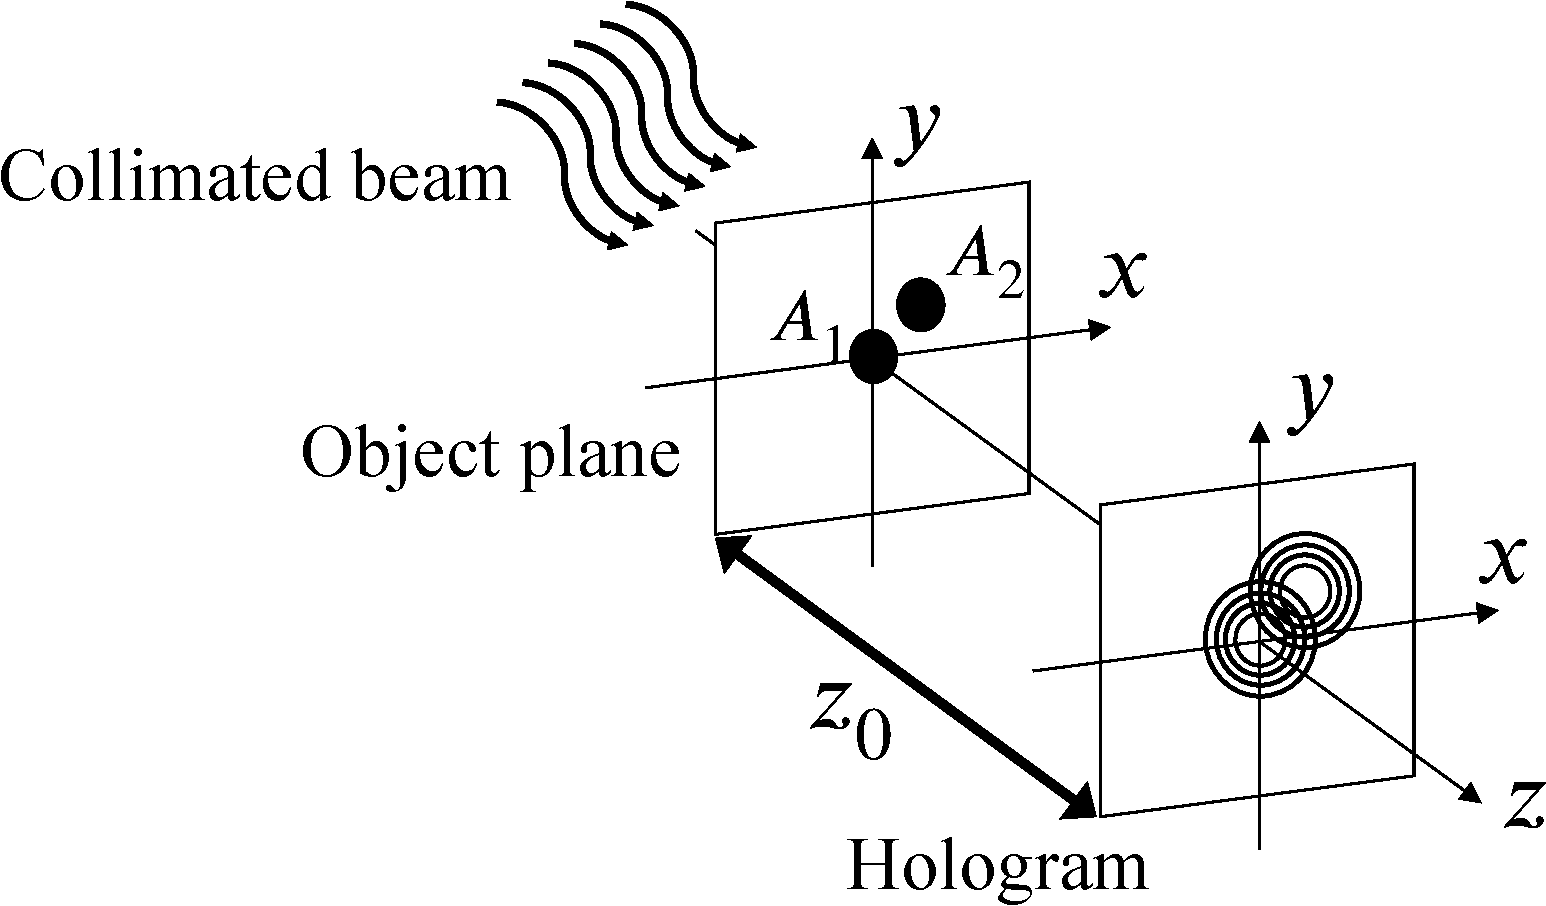
\includegraphics[width=0.8\linewidth]{./Figure/2_Theory/two_particle.pdf}
    \caption{Schematic of two-particle holography: two particles are located at $(0,0)$ and $(\Delta \xi, \Delta \eta)$, respectively. The depth position of the particles are the same, $z_{p1} = z_{p2}$.}
    \label{fig:twoParticleHolography}
\end{figure}

記録されるホログラム $I(x,y)$ は以下のように計算できる.
\begin{align}
    I(x,y) \coloneqq& \left|\psi_{A_1} + \psi_{A_2} - \psi_b \right|^2 \\
    \label{th:extraterms}
    =& |\psi_{A_1}|^2 + |\psi_{A_2}|^2 + 1 + 2\Re \left\{ \psi_{A_1} \overline{\psi_{A_2}} \right\} - 2\Re \left\{\overline{\psi_b}\left( \psi_{A_1} + \psi_{A_2} \right)\right\}
\end{align}
ここで,式(\ref{th:extraterms})右辺第3項以降を以下のように近似する.
\begin{equation}
    1 + 2\Re \left\{ \psi_{A_1} \overline{\psi_{A_2}} \right\} - 2\Re \left\{\overline{\psi_b}\left( \psi_{A_1} + \psi_{A_2} \right)\right\} = -1
\end{equation}
この近似の詳細については,付録\ref{sec:appendix_2particle}で述べる.結局,ホログラムは以下の式で与えられる.
\begin{equation}
    \label{th:2particleHologram}
    I(x,y) = |\psi_{A_1}|^2 + |\psi_{A_2}|^2 - 1
\end{equation}
したがって,同一物体面上同径近接粒子のホログラムは,二重露光ホログラフィで用いられていた以下の計算を適用可能になる\cite{doubleexposure}.

以降では,式(\ref{th:2particleHologram})に示したホログラムをフーリエ変換して得るスペクトル分布に現れる局所特徴について述べる.第一項および2項のフーリエ変換はそれぞれ以下で与えられる\cite{doubleexposure}.
\begin{align}
    \label{th:particle1Fourier}
    \varphi_{A_1}(\alpha,\beta)  = \mathcal{F}\left\{\left| \psi_{A_1} \right|\right\}  &\approx \cos{ \left( \pi \lambda z_0 \gamma^2 \right) }\tilde{A}(\alpha,\beta)  \\
    \label{th:particle2Fourier}
    \varphi_{A_2}(\alpha,\beta) = \mathcal{F}\left\{\left| \psi_{A_2} \right|\right\}   &\approx \cos{ \left( \pi \lambda z_0 \gamma^2 \right) }\tilde{A_2}(\alpha,\beta) \\
    &=\cos{ \left( \pi \lambda z_0 \gamma^2 \right) } \exp{\left( -2\pi \mathrm{j}\left( \alpha \Delta \xi + \beta \Delta \eta \right) \right)} \tilde{A}(\alpha,\beta)
\end{align}
ここで,$\tilde{A}$ は式(\ref{th:fourierOfA})を用いる.第二項のフーリエ変換 $\varphi_{A_2}$ の計算は,フーリエ変換のシフトルールによる.上の近似は,原点を除く点でのみ成立する.式(\ref{th:2particleHologram})第3項のフーリエ変換はデルタ関数であるため,これを省略して結局以下を得る.
\begin{align}
    \varphi(\alpha,\beta) &= \varphi_{A_1}(\alpha,\beta) + \varphi_{A_2}(\alpha,\beta) \\
    &= \tilde{A} \cos{\left( \pi \lambda z_0 \gamma^2 \right)} \cos{\left( \pi \left( \alpha \Delta \xi + \beta \Delta \eta \right) \right)} \exp{\left( \pi \mathrm{j} \left( \alpha \Delta \xi + \beta \Delta \eta \right) \right)}
\end{align}
したがって,スペクトル $S = |\varphi|^2$ は以下のようになる.
\begin{align}
    S(\alpha,\beta) &= \left| \varphi(\alpha,\beta) \right|^2 \\
    \label{th:2particleSpectrum}
    &= \left| \tilde{A} \right|^2 \cos^2{\left( \pi \lambda z_0 \gamma^2 \right)} \cos^2{\left( \pi \left( \alpha \Delta \xi + \beta \Delta \eta \right) \right)}
\end{align}
ここで,式(\ref{th:2particleSpectrum})の各因数の寄与を調べるために,数値生成したホログラムの例,ホログラムのスペクトル分布,同条件の式(\ref{th:2particleSpectrum})のプロットをFig. \ref{fig:2particleSpectrum}に示す.Fig. \ref{fig:2particleSpectrum:a}に示す物体面面像から式(\ref{th:lightProp_angularSpectrum})に示す光伝搬を用いてホログラムFig. \ref{fig:2particleSpectrum:b}を記録する.Fig. \ref{fig:2particleSpectrum:c}に示すスペクトルは,Fig. \ref{fig:2particleSpectrum:b}に対する高速フーリエ変換で得たものである.Fig. \ref{fig:2particleSpectrum:d}に示すスペクトルは,式(\ref{th:2particleSpectrum})を用いて計算したものである.式(\ref{th:2particleSpectrum})の因数 $\left| \tilde{A} \right|^2$ は,スペクトル分布において周期が変化しない同心円パターンとして現れている.これは,式(\ref{th:fourierOfA})に示す通り伝搬距離 $z_0$ に依存しないため,粒子の伝搬距離の変化に対してこのパターンは変化しない.Fig. \ref{fig:2particleSpectrum:d}では同心円パターンとして現れているが,Fig. \ref{fig:2particleSpectrum:c}では矩形領域に対する離散フーリエ変換の影響でパターンが歪んでいる.因数 $\cos^2{\left( \pi \lambda z_0 \gamma^2 \right)}$ は,スペクトル分布で確認できる残りの同心円パターンとして現れており,座標中心から離れるほど周期が短くなる.このパターンは,例に示す $z_0 = \SI{20}{\mm}$ 程度の小さな伝搬距離であれば確認できるが,一般的な記録条件で用いる伝搬距離ではエイリアシングによって確認できなくなる.最後に,因数 $\cos^2{\left( \pi \left( \alpha \Delta \xi + \beta \Delta \eta \right) \right)}$ はスペクトル分布の縞パターンを表す.このパターンは粒子組の平面内距離 $\Delta \xi$,$\Delta \eta$ に依存し,またこれらのみに依存するため,縞パターンの法線ベクトルから平面内距離を一意に決定できる.本節では同径かつ奥行方向距離を持たない2粒子のホログラムについて調べたが,半径が異なる場合,奥行方向距離を持つ場合のホログラフィックパターンについては付録\ref{sec:appendix_deviation}で述べる.

\begin{figure}[htbp]
    \centering
    \begin{subfigure}[b]{0.45\linewidth}
        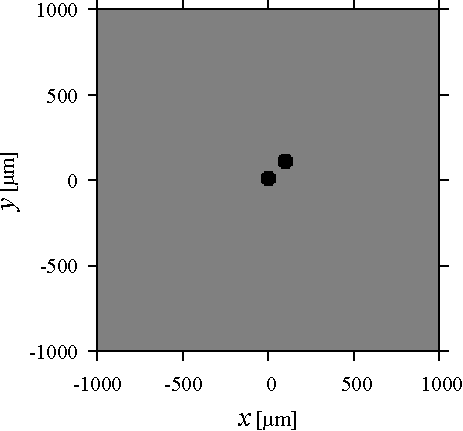
\includegraphics[width=\linewidth]{./Figure/2_Theory/spectrum_example/a.pdf}
        \caption{Object plane}
        \label{fig:2particleSpectrum:a}
    \end{subfigure}
    \hfill
    \begin{subfigure}[b]{0.45\linewidth}
        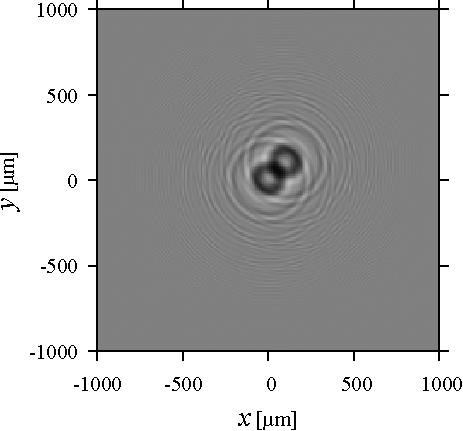
\includegraphics[width=\linewidth]{./Figure/2_Theory/spectrum_example/b.pdf}
        \caption{Recorded hologram}
        \label{fig:2particleSpectrum:b}
    \end{subfigure}

    \begin{subfigure}[b]{0.45\linewidth}
        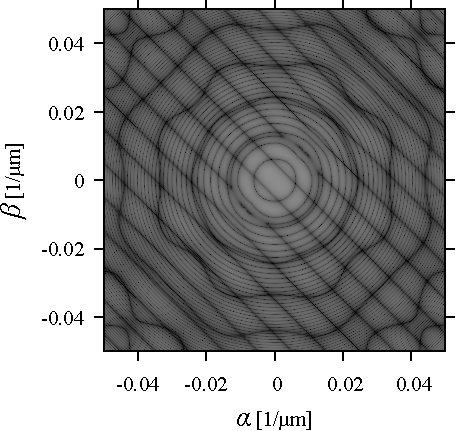
\includegraphics[width=\linewidth]{./Figure/2_Theory/spectrum_example/c.pdf}
        \caption{Computationally calculated spectrum of the hologram Fig. \ref{fig:2particleSpectrum:b}}
        \label{fig:2particleSpectrum:c}
    \end{subfigure}
    \hfill
    \begin{subfigure}[b]{0.45\linewidth}
        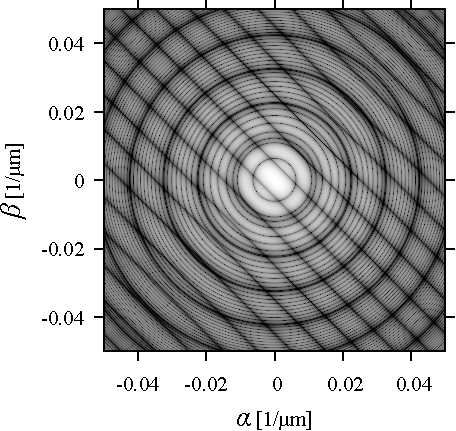
\includegraphics[width=\linewidth]{./Figure/2_Theory/spectrum_example/d.pdf}
        \caption{Spectrum of the hologram Fig. \ref{fig:2particleSpectrum:b} calculated by Eq. (\ref{th:2particleSpectrum})}
        \label{fig:2particleSpectrum:d}
    \end{subfigure}

    \caption{Example of a hologram and its spectrum. The radii of particles are $a_1 = a_2 = \SI{50}{\um}$. The propagation distance is $z_0 = \SI{20}{\mm}$. The distance between the centers of the particles is $\Delta \xi = \Delta \eta = \SI{100}{\um}$. The wavelength of the light is $\lambda = \SI{532}{\nm}$. The number of discrete points per side of the rectangular area to be Fourier transformed is 1024, and the pixel pitch is \SI{10}{\um}.} 
    \label{fig:2particleSpectrum}
\end{figure}

\subsubsection{離散スペクトル分布の縞パターンによる平面内距離の決定}
縞パターンの向き・および周期と平面内距離の関係が一意であることを\ref{sec:twoParticleHologram}節で示した.この節では,2粒子ホログラム画像のスペクトル分布上に現れる縞パターンから,粒子組の平面内距離 $(\Delta\xi,\Delta\eta)$ を決定する方法を示す.Fig. \ref{fig:stripePatternVector}に示すように縞パターンの状態を定義する.図中$\alpha$,$\beta$軸に沿って定義される離散点間隔 $l,\,m \mathrm{[pixel]}$ は,各軸の縞間隔である.図中では軸の次元と一致させるためにフーリエ変換を施す矩形領域一辺のピクセル長 $L \mathrm{\,[pixel]}$ とピクセルピッチ $\Delta x \mathrm{\,[\si{\um}]}$ の積で除している.
\begin{figure}[htbp]
    \centering
    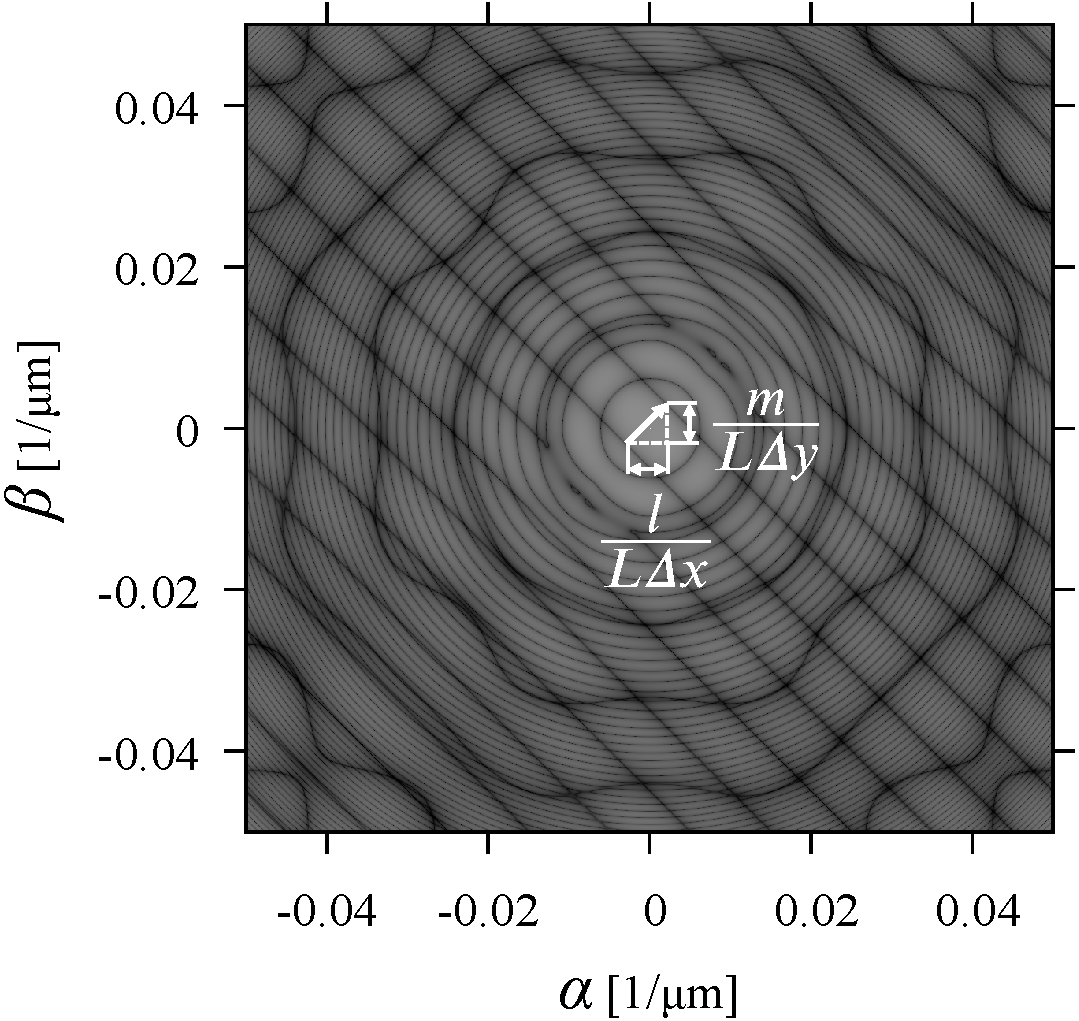
\includegraphics[width=0.8\linewidth]{./Figure/2_Theory/stripe_pattern.pdf}
    \caption{Schematic diagram defining the orientation and spacing of the stripe pattern using the displacements $l$ and $m$ along the $\alpha$ and $\beta$ axes. The displacement along each axis determines the characteristics of the stripe pattern and corresponds uniquely to the proximity state of the two particles}
    \label{fig:stripePatternVector}
\end{figure}

離散格子座標 $(x_i,y_i)$,$(\alpha_i.\beta_j)$ は,以下の関係を満たす.
\begin{align}
    \left( x_i, y_j \right) &= \left( i \Delta x, j \Delta x \right) \\
    \left( \alpha_i, \beta_j \right) &= \left( \frac{i}{L\Delta x}, \frac{j}{L\Delta x} \right)
\end{align}
以上の関係と,縞パターンの位相周期が $\pi$ であること,粒子組の接近角度と縞パターンの角度が等しいことから,以下の関係が成り立つ.
\begin{gather}
    \pi \left( \frac{l}{L\Delta x} \Delta \xi + \frac{m}{L\Delta x} \Delta \eta \right) = \pi \\
    \frac{\Delta \eta}{\Delta \xi} = \frac{m}{l}
\end{gather}
したがって,以下の関係を導出できる\cite{aem2023}.
\begin{equation}
    \label{th:stripepattern}
    \Delta \xi = \frac{lL\Delta x}{l^2+m^2}, \hspace{5mm} \Delta \eta = \frac{m L\Delta x}{l^2+m^2}
\end{equation}
$l$ および $m$ は $2 \leq l, m < L$ を満たす必要があるため,測定可能な平面内距離は以下の範囲に限られる.
\begin{equation}
    \Delta x \leq \Delta \xi < \frac{L\Delta x}{4}, \hspace{5mm} \Delta x \leq \Delta \eta < \frac{L\Delta x}{4}
\end{equation}

\subsection{畳み込みニューラルネットワークによる局所特徴識別}\label{sec:convolutionalNeuralNetwork}
\ref{sec:twoParticleHologramFeature}節において,近接粒子組のホログラムをそのスペクトル分布の局所特徴から識別可能であることを示した.本論文では,この原理を用いて,畳み込みニューラルネットワーク(Convolutional Neural Network: CNN)\cite{lecun1998}をベースとした画像認識モデルによって近接粒子組の識別を行う.このために本節では,画像認識モデルの学習・推論の原理と基本的な構造について示す.\ref{sec:supervisedClassification}節から\ref{sec:convolutionalLayer}までは機械学習の代表的なテキストであるBishop (2006)による\cite{bishop2006}.

\subsubsection{教師あり分類モデルの学習・推論}\label{sec:supervisedClassification}
教師あり分類モデルは,与えられたデータ $\bm{x}_i$ に対してそれが属する分類のクラス $C_k$ を推定する.本研究において,データのクラス数 $K$ はつねに2である.一般に深層学習を用いる識別モデルでは,データの正解ラベル $\bm{t}_i$,すなわちモデルが学習の後の推定結果として出力するのが望ましいデータは$K$次元ベクトルであり,例えばクラス1に属するデータの正解ラベルは以下のように表現される.
\begin{equation}
    \bm{t} = \left( 1, 0 \right)^\mathrm{T}
\end{equation}
実際のモデルの出力 $\bm{y}_i$ は,データがクラス1に属する確率 $p(C_1|\bm{x}_i)$ とクラス2に属する確率 $p(C_2|\bm{x}_i)$ を用いて以下のように表現される.
\begin{equation}
    \bm{y}_i = \left( p(C_1|\bm{x}_i), p(C_2|\bm{x}_i) \right)^\mathrm{T}
\end{equation}
$p(C_k|\bm{x}_i)$は,データ $\bm{x}_i$ 与えられた場合にそれがクラス $C_k$ に属する条件付き確率であり,データのクラス$C_k$の事後分布とも呼ばれる.これらは定義により以下の関係を満たす.
\begin{equation}
    \sum_{k=1}^K p(C_k|\bm{x}_i) = 1
\end{equation}
結局,教師あり分類モデルは,データ $\bm{x}_i$ に対してそのラベル $\bm{t}_i$ に十分近い出力 $\bm{y}_i$ を得るための関数 $f$ を決定する問題として定式化できる.
\begin{equation}
    \bm{y}_i = f(\bm{x}_i)
\end{equation}
$f$として3層のロジスティック回帰を用いる.各層$j = 1,2,3$の出力ベクトルを $\bm{\phi}_j$ とすると,各層について以下が成り立つ.
\begin{align}
    \bm{\phi}_1 &= \bm{x}_i \\
    \bm{\phi}_2 &= \sigma(\bm{W}_1 \bm{\phi}_1 + \bm{b}_1) \\
    \bm{\phi}_3 &= \sigma(\bm{W}_2 \bm{\phi}_2 + \bm{b}_2) \\
    \bm{y}_i &= \bm{\phi}_3
\end{align}
$\bm{W}_j$は$\mathrm{dim}\bm{\phi}_{j+1}\times \mathrm{dim}\bm{\phi}_{j}$型の係数行列を表し,$\bm{b}$は各層のバイアスベクトルを表す.$\sigma$はシグモイド関数であり,以下で定義される.
\begin{equation}
    \sigma(x) = \frac{1}{1+\exp{(-x)}}
\end{equation}
このように,入力層 $\bm{\phi}_1$,中間層 $\bm{\phi}_2$,出力層 $\bm{\phi}_3$ からなるモデルを順伝播型ニューラルネットワークと呼ぶ.このようなモデルは,中間層の出力ベクトル $\bm{\phi}_2$の次元を十分大きく取れば $f$と同型の任意の非線形関数を近似することができることが知られている\cite{cybenko1989}.実際の深層学習モデルでは中間層は1層ではなく複数の層からなる場合があり,さらに活性化関数としてシグモイド関数ではなくReLU関数\cite{nair2010}などを用いる場合があるが,これらは計算の効率化や学習の安定化のための工夫であり,本質的には同じモデルである.


このモデルの学習は,データ $\bm{x}_i$ と正解ラベル $\bm{t}_i$ を用いて,以下の損失関数 $E$ を最小化することで行われる.
\begin{equation}
    \label{th:lossFunction}
    E(\bm{W}_1,\bm{W}_2,\bm{b}_1,\bm{b}_2) = -\sum_{i=1}^N \sum_{k=1}^K t_{ik} \ln{y_{ik}}
\end{equation}
上式は交差エントロピー誤差と呼ばれ,二項分類問題における標準的な損失関数である.$N$はデータ数である.この損失関数を最小化するパラメータ $\bm{W}_1,\bm{W}_2,\bm{b}_1,\bm{b}_2$ を求めるために,勾配降下法を用いる.勾配降下法は,損失関数の勾配を用いて,パラメータを以下のように更新する.
\begin{equation}
    \bm{W}_j \leftarrow \bm{W}_j - \eta \frac{\partial E}{\partial \bm{W}_j}, \hspace{5mm} \bm{b}_j \leftarrow \bm{b}_j - \eta \frac{\partial E}{\partial \bm{b}_j}
\end{equation}
上式は更新率$\eta $をパラメータに取る最も単純な勾配降下式であるが,実際の深層学習モデルではAdam\cite{kingma2015}などの高度な勾配降下法が用いられる.勾配降下法によるパラメータ更新を繰り返すことで,損失関数を最小化するパラメータを求めることができる.


\subsubsection{畳み込み層による特徴抽出}\label{sec:convolutionalLayer}
画像などの2次元データに対して,ロジスティック回帰層を重ねて得られる全結合ニューラルネットワークを用いて識別を行うと,所望の精度を得るために必要なパラメータ数が非常に多くなる.画像の局所特徴を効率よく抽出する仕組みとして畳み込み層\cite{lecun1998}が提案され,これを用いた画像認識モデルであるAlexNet\cite{krizhevsky2012}が高い性能を示したことで現在に至るまで画像認識モデルの基本的な構造として用いられている.画像認識モデルでは,入力層に近い層で複数の畳み込み層による処理が行われ,特徴抽出・次元削減が行われた後,全結合層に接続し識別を行う.本節では,畳み込み層の原理と構造について示す.

畳み込み層における処理は,カーネルによる畳み込み計算,活性化関数による非線形化,部分サンプリングで構成される.カーネルはカーネルサイズを $L_{k}$ として $L_k \times L_k$ の実数配列であり,二次元データ $\bm{X}_i$ のすべての可能な $L_k \times L_k$ サイズの部分配列と要素ごとの積和を計算する.これらを並べてできる二次元配列 $\bm{Y}_i$ が出力のあるチャネル部分に相当する.データ $\bm{X}_i$ の一辺のデータ数を $L$ としたとき,チャネル出力 $\bm{Y}_i$ の一辺のデータ数は $L-L_k+1$ となるか,あらかじめデータ $\bm{X}_i$ の境界を$L_k$ だけゼロパディングしておくことで $L$ となる.カーネル演算の後に$\bm{Y}_i$と同型のバイアス配列を加える場合もある.これに活性化関数を適用することで,出力 $\bm{Y}_i$ の各要素は以下のように表現できる.
\begin{equation}
    \bm{Y}_i = \sigma \left( \bm{W} \ast \bm{X}_i + \bm{A} \right)
\end{equation}
ひとつの畳み込み層では一般に複数のカーネルを定義し,それぞれのカーネルによる畳み込み計算を行う.畳み込み層への入力データのチャネル数を $C$,カーネル数を $n$ とすると,入力データ・出力データの関係はFig. \ref{fig:convolutionalLayer}に示すようになる.
\begin{figure}[htbp]
    \centering
    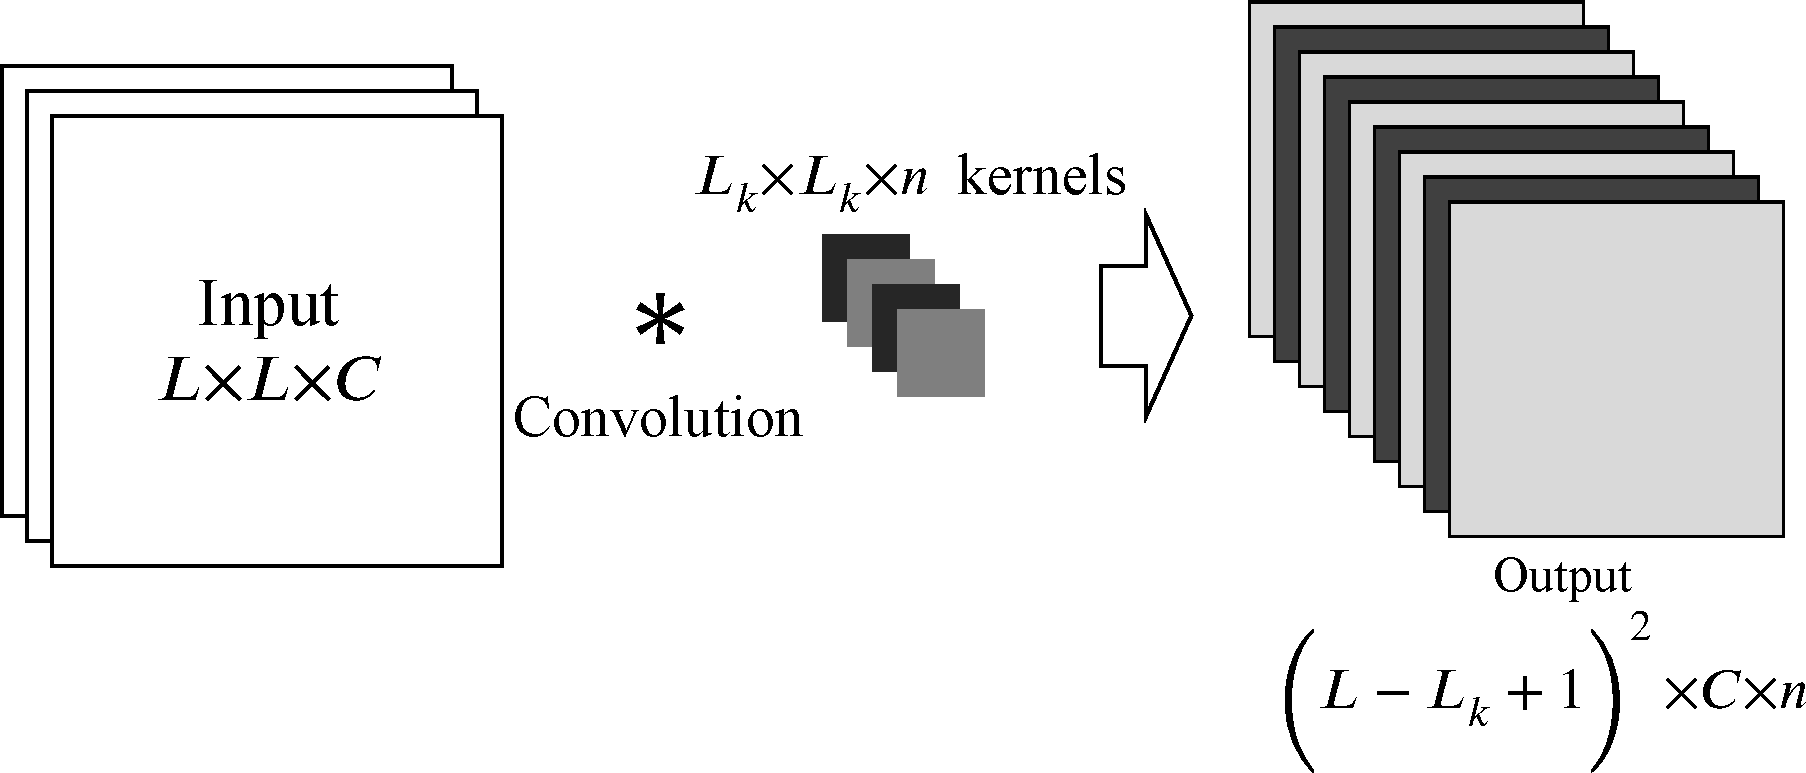
\includegraphics[width=0.8\linewidth]{./Figure/2_Theory/cnn.pdf}
    \caption{Schematic diagram of a convolutional layer. The input data $\bm{X}_i$ is a $C\times L \times L$ array, and the output data $\bm{Y}_i$ is a $C\times n\times (L-L_k+1) \times (L-L_k+1)$ array.}
    \label{fig:convolutionalLayer}
\end{figure}

多くの畳み込みニューラルネットワークでは,畳み込み層のあとにプーリング層を挿入する.プーリング層は,入力データの局所的な特徴を保持しつつデータのサイズを小さくするために用いられる.プーリング層では,入力データの局所的な特徴を保持するために,入力データの局所的な領域に対して最大値や平均値を計算する.これらの演算は,入力データのチャネルごとに行われる.プーリング層の出力データのチャネル数は入力データのチャネル数と同じである.プーリング層の出力データのサイズは,入力データのサイズをプーリングサイズで割った商である.最もよく用いられるプーリング処理としてMax-Pooling\cite{nagi2011}がある.これは,入力データの局所的な領域に対して最大値を計算しその領域の代表値とする処理である.$2\times 2$のMax-Poolingを行う場合,出力データのサイズは入力データの半分になる.


\subsubsection{先進的な画像認識モデルとその構造}
AlexNet\cite{krizhevsky2012}の登場以降,VGG (2015)\cite{simonyan2015},ResNet (2016)\cite{he2016},Vision Transformer (2021)\cite{dosovitskiy2021},EffcientNetV2 (2021)\cite{tan2021}などの代表的な画像認識モデルが提案されている.VGGは畳み込み層を用いた大きなモデルの実装により現在でも多くの物体検出モデルの基幹モデルとして採用されている.ResNetはニューラルネットワークの隣接しない層同士を接続するSkip connectionの導入によって大きく精度を向上させた.Vision TransformerはCNNベースではなくTransformer\cite{vaswani2017}ベースのモデルだが,現在に至るまで画像認識モデルの性能評価の基準として用いられている.EfficientNetV2は再びCNNベースのモデルであり,現在のState-of-the-artなモデルとしてデファクトで用いられている.本研究でも,EffcientNetV2を用いて画像認識を行う.

これらのモデルに共通する特徴として,公開されている大規模画像データベースであるImageNet\cite{deng2009}による事前学習を行い,その後識別したいドメインのデータで学習を行っている点である.ImageNetは,\num{21000}クラス以上,\num{1400}万枚の画像からなるデータベースであり,設計したモデルをImageNetで事前学習することで,畳み込み層のパラメータは像の局所特徴を抽出するように最適化される.事前学習したモデルの畳み込み層部分を切り取りその末尾に全結合層を追加し,識別したいドメインのデータで学習を行うことで,識別したいドメインのデータに特化したモデルを得ることができる.これを転移学習\cite{zhuang2020}という.本研究でも,ImageNetで事前学習したEfficientNetV2を用いて転移学習を行う.モデルの構成,学習データ生成,学習方法などの詳細については\ref{sec:EffNetV2}節で示す.


\subsection{位相回復ホログラフィによる水滴像の3次元再生}
この節では,近接粒子の近接検出を行う画像認識モデルを用いて抽出された近接粒子組ホログラムに対して実際に光伝搬計算による3次元像再生を行うときに用いる位相回復ホログラフィについて説明する.まず,位相回復ホログラフィの原理について示し,次に\ref{sec:holographyBottleNeck}節で示したGaborホログラフィによる再生像品質の低下が改善されることを示す.最後に,改善した粒子輝度値の奥行方向プロファイルから粒子の奥行方向位置を決定する手法について示す.

\subsubsection{位相回復ホログラフィの原理}\label{sec:phaseRetrieval}
位相回復ホログラフィ\cite{phaseretrieval}では,物体面からの伝搬距離が異なる二枚のインラインホログラム,すなわち光強度分布を用いて失われた位相分布を復元する\cite{zhang2003,tanaka2016}.このために,同光軸上の2カメラで記録されたホログラムに対してGerchberg-Saxtonアルゴリズム\cite{gerchberg1972}を適用する.物体面から記録面1までの伝搬距離を $z_1$,さらに記録面1から記録面2までの伝搬距離を $\Delta z$ としたときの物体面と各記録ホログラムの関係をFig. \ref{fig:phaseRetrievalOptics}に示す.
\begin{figure}[htbp]
    \centering
    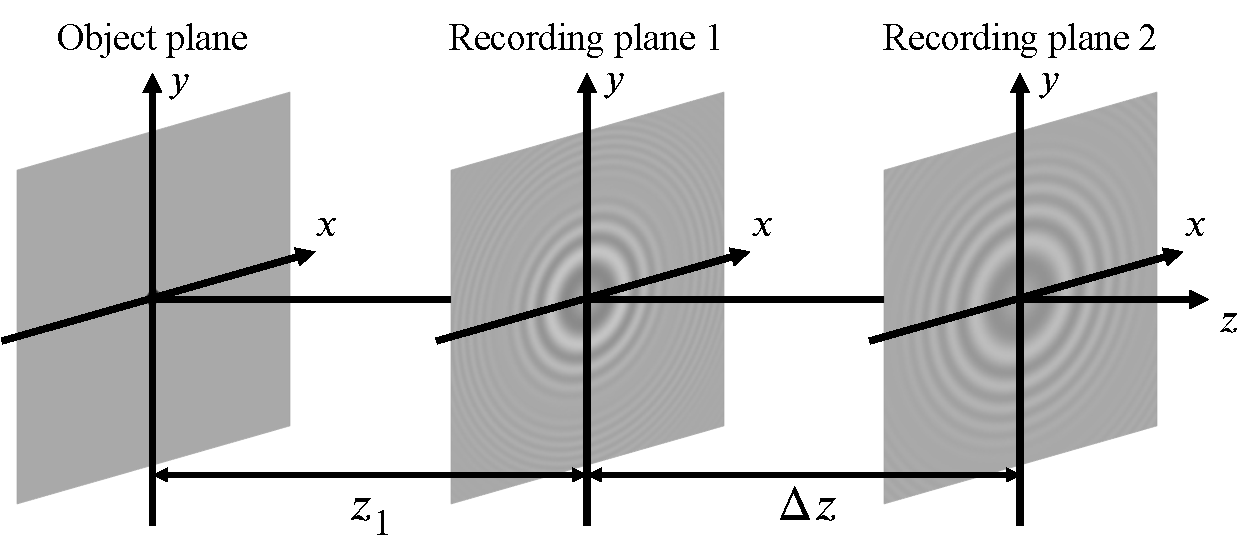
\includegraphics[width=0.8\linewidth]{./Figure/2_Theory/pralignment.pdf}
    \caption{Optical system for phase retrieval holography. The object plane is located at $z = 0$. The distance between the object plane and the first recording plane is $z_1$, and the distance between the first and second recording planes is $\Delta z$.}
    \label{fig:phaseRetrievalOptics}
\end{figure}
位相分布ホログラフィでは,以下の反復計算によって記録面1における複素振幅 $\psi_1$ を復元する.ここで,各記録面$i=1,2$におけるホログラムを$I_i$,$n$回目の反復計算で得た複素振幅を $\psi_i^n$,位相分布を $\phi_i^n$ とし,これらの初期条件$\psi_1^1$および$\phi_1^1$を以下で定める.
\begin{equation}
    \phi_1^1 = 0,  \quad \psi_1^1 = \sqrt{I_i} \exp{(i\phi_i^0)}
\end{equation}
以下の計算ステップに従い $\phi_1^n$ を得る.


\paragraph{STEP 1:}
\begin{equation}
    \psi_2^n = \psi_1^n * h_{\Delta z}
\end{equation}
\begin{equation}
    \phi_2^{n} = \arctan{\left( \frac{\Im \psi_2^n}{\Re \psi_2^n} \right)}
\end{equation}
$\psi_1^n$を記録面2の位置まで伝搬した複素振幅を$\psi_2^n$とする.$\psi_2^n$を用いて記録面2における位相分布 $\phi_2^n$ を計算する.

\paragraph{STEP 2:}
\begin{equation}
    \psi_2^n = \sqrt{I_2} \exp{(\mathrm{j}\phi_2^n)}
\end{equation}
STEP 1で得た位相分布 $\phi_2^n$ を用いて記録面2における複素振幅 $\psi_2^n$ を計算する.$\psi_2^n$の実振幅を$\sqrt{I_2}$で拘束する.

\paragraph{STEP 3:}
\begin{equation}
    \psi_1^{n+1} = \psi_2^n * h_{-\Delta z}
\end{equation}
\begin{equation}
    \phi_1^{n+1} = \arctan{\left( \frac{\Im \psi_1^{n+1}}{\Re \psi_1^{n+1}} \right)}
\end{equation}
STEP 2で得た複素振幅 $\psi_2^n$ を記録面1の位置まで伝搬した複素振幅を$\psi_1^{n+1}$とする.$\psi_1^{n+1}$を用いて記録面1における位相分布 $\phi_1^{n+1}$ を計算する.

\paragraph{STEP 4:}
\begin{equation}
    \psi_1^{n+1} = \sqrt{I_1} \exp{(\mathrm{j}\phi_1^{n+1})}
\end{equation}
STEP 3で得た位相分布 $\phi_1^{n+1}$ を用いて記録面1における複素振幅 $\psi_1^{n+1}$ を計算する.$\psi_1^{n+1}$の実振幅を$\sqrt{I_1}$で拘束する.

\vspace{10pt}
以上の計算を繰り返すことで,記録面1における複素振幅 $\psi_1$ を得る.ふたつの記録ホログラム間距離$\Delta z$は以下の式から決定する\cite{tanaka2016}.
\begin{equation}
    \Delta z = \frac{z_1}{m}, \quad ( m = 1,2,3,\cdots )
\end{equation}

\subsubsection{位相回復ホログラフィによる再生像品質の改善}
位相回復ホログラフィによって粒子再生像がGaborホログラフィからどのように改善するか示す.まず,Fig. \ref{fig:twinImage}に示す系の位相回復ホログラフィによる再生像とその輝度プロファイルをFig. \ref{fig:twinImagePR}に示す.Fig. \ref{fig:twinImage:holo}に見られた双画像によるホログラムフリンジはほとんど消失し,Fig. \ref{fig:twinImage:profile}に示すように粒子位置での輝度値が0となりもとの粒子形状関数をよく再現していることがわかる.
\begin{figure}[htbp]
    \centering
    \begin{subfigure}[t]{0.48\linewidth}
        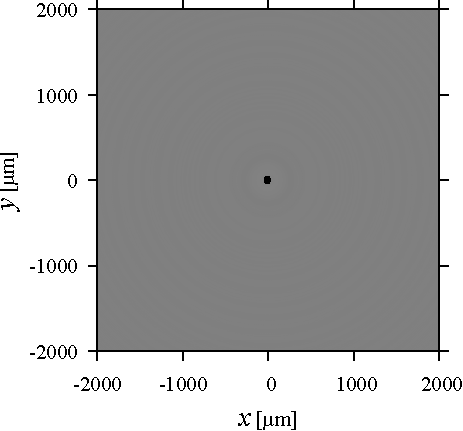
\includegraphics[width=\linewidth]{./Figure/2_Theory/PR_twin_image/prrec.pdf}
        \caption{Reconstructed image of hologram using phase retrieval holography.}
        \label{fig:twinImagePR:holo}
    \end{subfigure}
    \hfill
    \begin{subfigure}[t]{0.48\linewidth}
        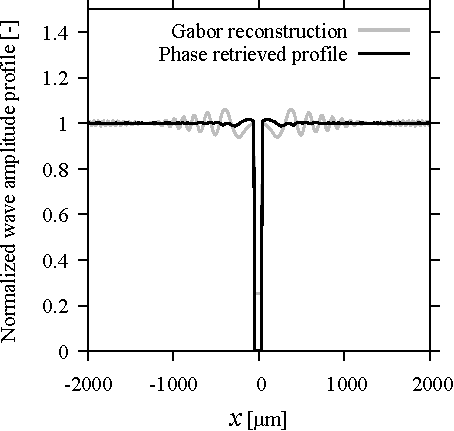
\includegraphics[width=\linewidth]{./Figure/2_Theory/PR_twin_image/prprofile.pdf}
        \caption{Normalized wave amplitude profile of reconstructed images of phase retrieved hologram and gabor hologram along the line $y=\SI{0}{\um}$ }
        \label{fig:twinImagePR:profile}
    \end{subfigure}

    \caption{Example of a reconstructed image slice of phase retrieved hologram and its wavefront irradiance profile. The hologram is recorded at $z=\SI{80}{\mm}$, and the image slice is reconstructed at $z=\SI{0}{\mm}$. The particle radius is $a=\SI{50}{\um}$, and the recording wavelength is $\lambda = \SI{632.8}{\nm}$. The distance between the two recording planes is $\Delta z = \SI{40}{\mm}$, and the phase retrieving iteration number is $n=10$. The phase retrieved profile well reproduces the original particle shape: the twin image is suppressed, and the irradiance value on the particle is equal to 0 as in the original particle shape.}
    \label{fig:twinImagePR}
\end{figure}

次に,奥行方向への像伸びについて示す.Fig. \ref{fig:particlePRZprofile} にGabor再生,位相回復ホログラフィによる再生,式(\ref{th:particleZprofile})による$z$軸方向正規化輝度プロットを示す.Gabor再生像では粒子位置周辺で輝度値が0にならないため位置検出が困難であったが,位相回復ホログラフィによる再生プロファイルでは粒子位置周辺で輝度値が0となる.式(\ref{th:elongationLength})における$m=3$相当の像伸びを確認できる.この$z$軸輝度プロファイルから,粒子の奥行方向位置を決定する手法について\ref{sec:particleDepth}節で示す.
\begin{figure}[htbp]
    \centering
    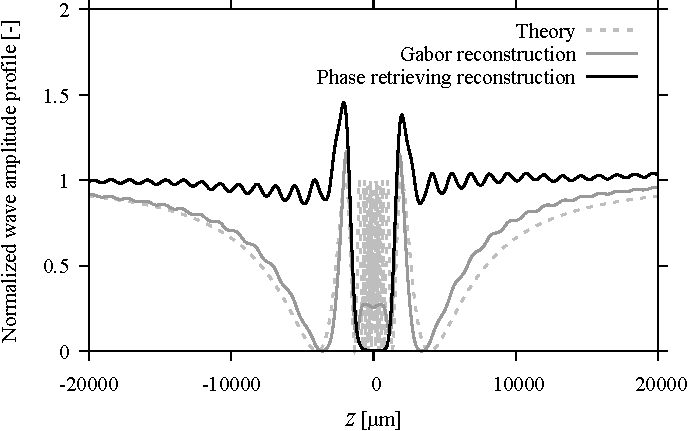
\includegraphics[width=0.8\linewidth]{./Figure/2_Theory/przprofile.pdf}
    \caption{Normalized $z$-axis irradiance profile of phase retrieved hologram, Gabor hologram and theoretical plot of Eq. (\ref{th:particleZprofile}). The hologram is recorded at $z = \SI{0}{\um}$, particle radius is $a=\SI{50}{\um}$, and the recording wavelength is $\lambda = \SI{632.8}{\nm}$. The same system used in Fig. \ref{fig:twinImagePR} is used for this calculation.}
    \label{fig:particlePRZprofile}
\end{figure}

\subsubsection{粒子奥行位置決定手法}\label{sec:particleDepth}
Fig. \ref{fig:particlePRZprofile}に示すように,位相回復ホログラフィによる再生像では,粒子の真の奥行位置を含む広い領域で輝度値が0となる.奥行方向位置を一点に決定するために,Tamuraの方法を用いる\cite{memmolo2011}.Tamuraの方法では,以下の評価関数 $C^2(z;x,y)$ を最大化するような$z$を求める.
\begin{equation}
    \label{th:tamura}
    C^2(z;x,y) = \frac{\sigma{\left( \bm{I}|_z \right)}}{\mu{\left( \bm{I}|_z \right)}}
\end{equation}
$\sigma$,$\mu$はそれぞれ標準偏差,平均値を示す.$\bm{I}|_z$は,ある奥行位置$z$における再生像$I_z$のうち,$x$-$y$平面内の粒子中心$(x,y)$近傍の粒子像を含む部分画像を示す.このようにして決定された $z$ の解像度は,ホログラムの奥行方向再生解像度$\Delta z$と等しい.

Fig. \ref{fig:tamuratheory}に,Fig. \ref{fig:particlePRZprofile}に示す位相回復した再生像の粒子中心$z$軸プロファイルと,式(\ref{th:tamura})に示すプロットを示す.$\bm{I}|_z$は,粒子像をちょうど包含する$2r_p \times 2r_p$の領域に対して計算する.$C^2$が最大値を取る$z$を奥行粒子位置として決定できることがわかる.
\begin{figure}[H]
    \centering
    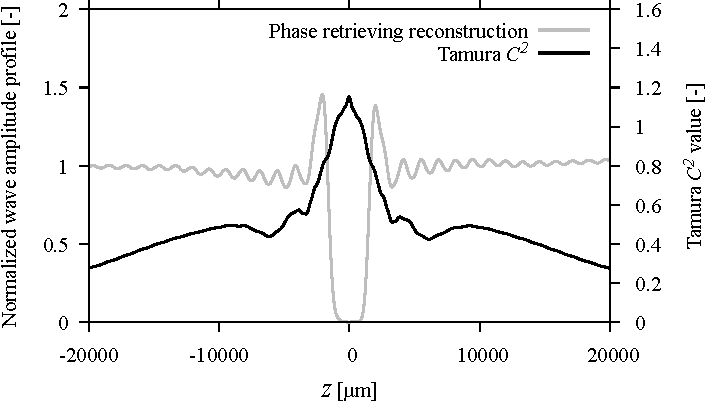
\includegraphics[width=0.8\linewidth]{./Figure/2_Theory/tamuraprof.pdf}
    \caption{Tamura $C^2$ function plot of the reconstructed image of phase retrieved hologram. The hologram is recorded at $z = \SI{0}{\um}$, particle radius is $a=\SI{50}{\um}$, and the recording wavelength is $\lambda = \SI{632.8}{\nm}$. The same system used in Fig. \ref{fig:twinImagePR} is used for this calculation.}
    \label{fig:tamuratheory}
\end{figure}



\newpage
\section{2粒子ホログラムの局所特徴}
この節では,



\subsection{実験による検証}














\newpage
\section{方法}
\subsection{近接2粒子ホログラムの検証実験}
\subsection{実験装置}
\subsection{EffcientNetV2モデルの学習}
\newpage
\section{結果}

\newpage
\section{結論}
















\newpage
\section*{謝辞}
\addcontentsline{toc}{section}{\gt 謝辞}
\newpage
\section*{筆頭論文}
\addcontentsline{toc}{section}{\gt 筆頭論文}

\begin{description}
    \item[(Paper1)] Nakai, D., and Tanaka, Y., “In-Line Digital Holographic Reconstruction by Using GPU Programming with Python”, Advanced Experimental Mechanics, 7, pp.169-173, (2022).
    \item[(Paper2)] Nakai, D., and Tanaka, Y., “Spatial Frequency Analysis of Holograms of Two Droplets in Close Proximity”, Advanced Experimental Mechanics, 8, pp.33-38, (2023).
\end{description}
\section*{受賞}
\addcontentsline{toc}{section}{\gt 受賞}
\begin{description}
    \item[(Award1)] 中井大,ベストプレゼンテーション賞,“微小液滴ホログラムのためのCNNベース衝突検知モデルの評価”,可視化情報学会 第50回可視化情報シンポジウム, 東京 工学院大学, 2021/8.
    \item[(Award2)] Nakai, D., Outstanding Oral Presentation Award, “Effect of Depth-Position Displacement of Approaching Microdroplet Pairs on Holographic Patterns”, International Workshop on Advanced Experimental Mechanics for Students and Young Researchers 2022, A050, Online, Nov. 2022.
\end{description}
\section*{国際学術会議}
\addcontentsline{toc}{section}{\gt 国際学術会議}

\begin{enumerate}
\renewcommand{\labelenumi}{(\arabic{enumi})}
    \item Nakai, D., and Tanaka, Y., “Study on a Holographic Pattern and its Spectral Distribution Formed by Two Approaching Spheres”, The 32nd International Symposium on Imaging, Sensing, and Optical Memory, C000607, Sapporo, Aug. 2022.
    \item Nakai, D., and Tanaka, Y., “Effect of Depth-Position Displacement of Approaching Microdroplet Pairs on Holographic Patterns”, International Workshop on Advanced Experimental Mechanics for Students and Young Researchers 2022, A050, Online, Nov. 2022.
    \item Nakai, D., and Tanaka, Y., “Measurement of Nanoliter Droplets in a Microchannel Using Phase Retrieval Holography”, The 11th International Conference on Multiphase Flow, \#790, Kobe, Nov. 2022.
    \item Nakai, D., and Tanaka, Y., “Holographic Collision Analysis of Microdroplets: Data Augmentation with OpenFOAM”, ASME-JSME-KSME Fluids Engineering Division 2023, \#3-09-1-04, Osaka, Jul. 2023.
    \item Nakai, D., and Tanaka, Y., “Recognition of Approaching Droplet Holograms using Image Recognition Models”, International Workshop on Advanced Experimental Mechanics for Students and Young Researchers 2023, A042, Osaka, Nov. 2023.
\end{enumerate}

\section*{国内学術会議}
\addcontentsline{toc}{section}{\gt 国内学術会議}
\begin{description}
    \item[(O1)] 中井 大, 田中 洋介, “機械学習に基づく時系列ホログラムの微小液滴衝突検知”, 日本機械学会 関西学生会2021年度学生員卒業研究発表講演会, SS3-(13)-3, 2022/3,(オンライン口頭発表)発表日:2022年3月15日
    \item[(O2)] 中井 大, 田中 洋介, “微小液滴ホログラムのためのCNNベース衝突検知モデルの評価”, 可視化情報学会 第50回可視化情報シンポジウム, 東京 工学院大学, 2021/8. 発表日:2022年8月8日
    \item[(O3)] 中井 大, 田中 洋介, “インライン位相回復ホログラフィによるボールレンズの形状計測”, 日本実験力学会 2022年度年次講演会, 鳥取 鳥取大学, 2021/08. 発表日:2022年8月24日
    \item[(O4)] 中井 大, 田中 洋介, “液滴衝突における2液滴間距離がホログラフィックパターンに与える影響”, 日本光学会年次学術講演会 Optics \& Photonics Japan 2022, 栃木 宇都宮大学, 2022/11. 発表日:2022年11月13日
    \item[(P5)] 中井 大, 田中 洋介, “機械学習を用いたマイクロ液滴近接検出”, 日本機械学会関西支部 第98期定時総会講演会, 京都 京都工芸繊維大学, 2023/03. 発表日:2023年3月16日
    \item[(O6)] 中井 大, 田中 洋介, “Julia × GPU によるホログラフィック微粒子計測”, 日本実験力学会 光学的手法分科会研究会, つくば 産総研つくばセンター, 2023/07. 発表日:2023年7月4日
    \item[(O7)] 中井 大, 田中 洋介, “奥行方向距離を持つ近接液滴組のホログラフィックパターンとそのスペクトル分布に関する実験的研究”, 日本実験力学会 2023年度年次講演会, 和歌山 和歌山城ホール, 2023/08. 発表日:2023年8月29日
    \item[(O8)] 中井 大, 田中 洋介, “GPU搭載シングルボードコンピュータと2台のカメラによるリアルタイム位相回復ホログラフィ再生処理モジュールの開発”, 高速度イメージングとフォトニクスに関する総合シンポジウム2023, 東大阪 近畿大学, 2023/12. 発表日:2023年12月14日
\end{description}
\newpage
\bibliography{refs}
\addcontentsline{toc}{section}{\gt 参考文献}
\newpage
\appendix
\section*{付録}
\addcontentsline{toc}{section}{付録}

\renewcommand{\thesubsection}{\Alph{subsection}}
\subsection{2粒子ホログラムの近似}
\label{sec:appendix_2particle}

\subsection{異径・奥行方向距離を持つ場合の2粒子ホログラム}
\label{sec:appendix_deviation}


\subsubsection{奥行方向距離を持たない異径粒子組についてのメモ}
AEMでは,粒子1が記録されたときの複素振幅を $\psi_1$,粒子2を $\psi_2$として,
\begin{equation}
    I(x,y) = |\psi_1|^2 + |\psi_2|^2 -1
\end{equation}
が成り立つと仮定した.さらに,
\begin{equation}
    \varphi_1(\alpha,\beta) = \mathcal{F}\{|\psi_1|^2\} \approx \cos{(\pi \lambda z_0 \gamma^2)} \tilde{A_1}
\end{equation}
\begin{align}
    \varphi_2(\alpha,\beta) = \mathcal{F}\{|\psi_2|^2\} &\approx \cos{(\pi \lambda z_0 \gamma^2)} \tilde{A_2} \\
    &= \cos{(\pi \lambda z_0 \gamma^2)} \exp{(-2\pi \mathrm{j} (\alpha \Delta \xi + \beta \Delta \eta))} \tilde{A'_2}
\end{align}
が成り立つ.ただし, $A'_2$は,粒子1とことなる粒径を持つ粒子2が,粒子1同様原点中心になるときの形状関数である.つまり,以下の関係を満たす.
\begin{equation}
    A'_2(x-\Delta \xi, y- \Delta \eta ) = A_2
\end{equation}
ここで,粒子1の粒径を $a$ ,粒子2の粒径を $a+\Delta a$ とすると, $\tilde{A_1}$および $\tilde{A_2}$ はそれぞれ
\begin{equation}
    \tilde{A_1}(\alpha,\beta) = a \frac{J_1(2\pi a \gamma)}{\gamma}
\end{equation}
\begin{equation}
    \tilde{A'_2}(\alpha,\beta) = (a+ \Delta a) \frac{J_1(2\pi (a + \Delta a) \gamma)}{\gamma}
\end{equation}
となる. $\tilde{A'_2}$ を $\tilde{A_1}$ によって表現できたら,AEMで論じた以下の式と剰余項の和として扱える.
\begin{align}
    \varphi &= \varphi_1(\alpha,\beta) + \varphi_2(\alpha,\beta) \\
    &= \tilde{A_1} \cos{(\pi \lambda z_0 \gamma^2) \cos{(\pi  (\alpha \Delta \xi + \beta \Delta \eta))}}\exp{(\pi \mathrm{j} (\alpha \Delta \xi + \beta \Delta \eta))} + O
\end{align}

\begin{equation}
    v_{\theta} = \frac{C}{2\pi r} \left( 1- \exp{\left(-\frac{Ar^2}{2\nu}\right)} \right)
\end{equation}
\end{document}
